%%%%%%%%%%%%%%%%%%don't forget if needed %%%%%%%%%%%%%%%%%%%%%
%\section[toc version]{title version%
%              \sectionmark{head version}}
%\sectionmark{head version}
%%%%%%%%%%%%%%%%%%%%%%%%%%%%%%%%%%%%%%%%%%%%%%%%%%%%%%%%%%%%%%
\def\titcourt{Numerical comparison of basal and lateral melting of phase change material}
\def\titlong{Numerical comparison of basal and lateral melting of phase change material}
%%%%%%%%%%%%%%%%%%%%%%%%%%%%%%%%%%%%%%%%%%%%%%%%%%%%%%%%%%%%%%%%
\chapter[\titlong]{\titlong%
              \chaptermark{\titcourt}}
\chaptermark{\titcourt}
\label{chap-MELTING-ANALYSIS}
%%%%%%%%%%%%%%%%%%%%%%%%%%%%%%%%%%%%%%%%%%%%%%%%%%%%%%%%%%%%%%%%
%%%%%%%%%%%%%%%%%%%%%%%%%%%%%%%%%%%%%%%%%%%%%%%%%%%%%%%%%%%%%%%%
\begin{figure}
	\begin{center}
		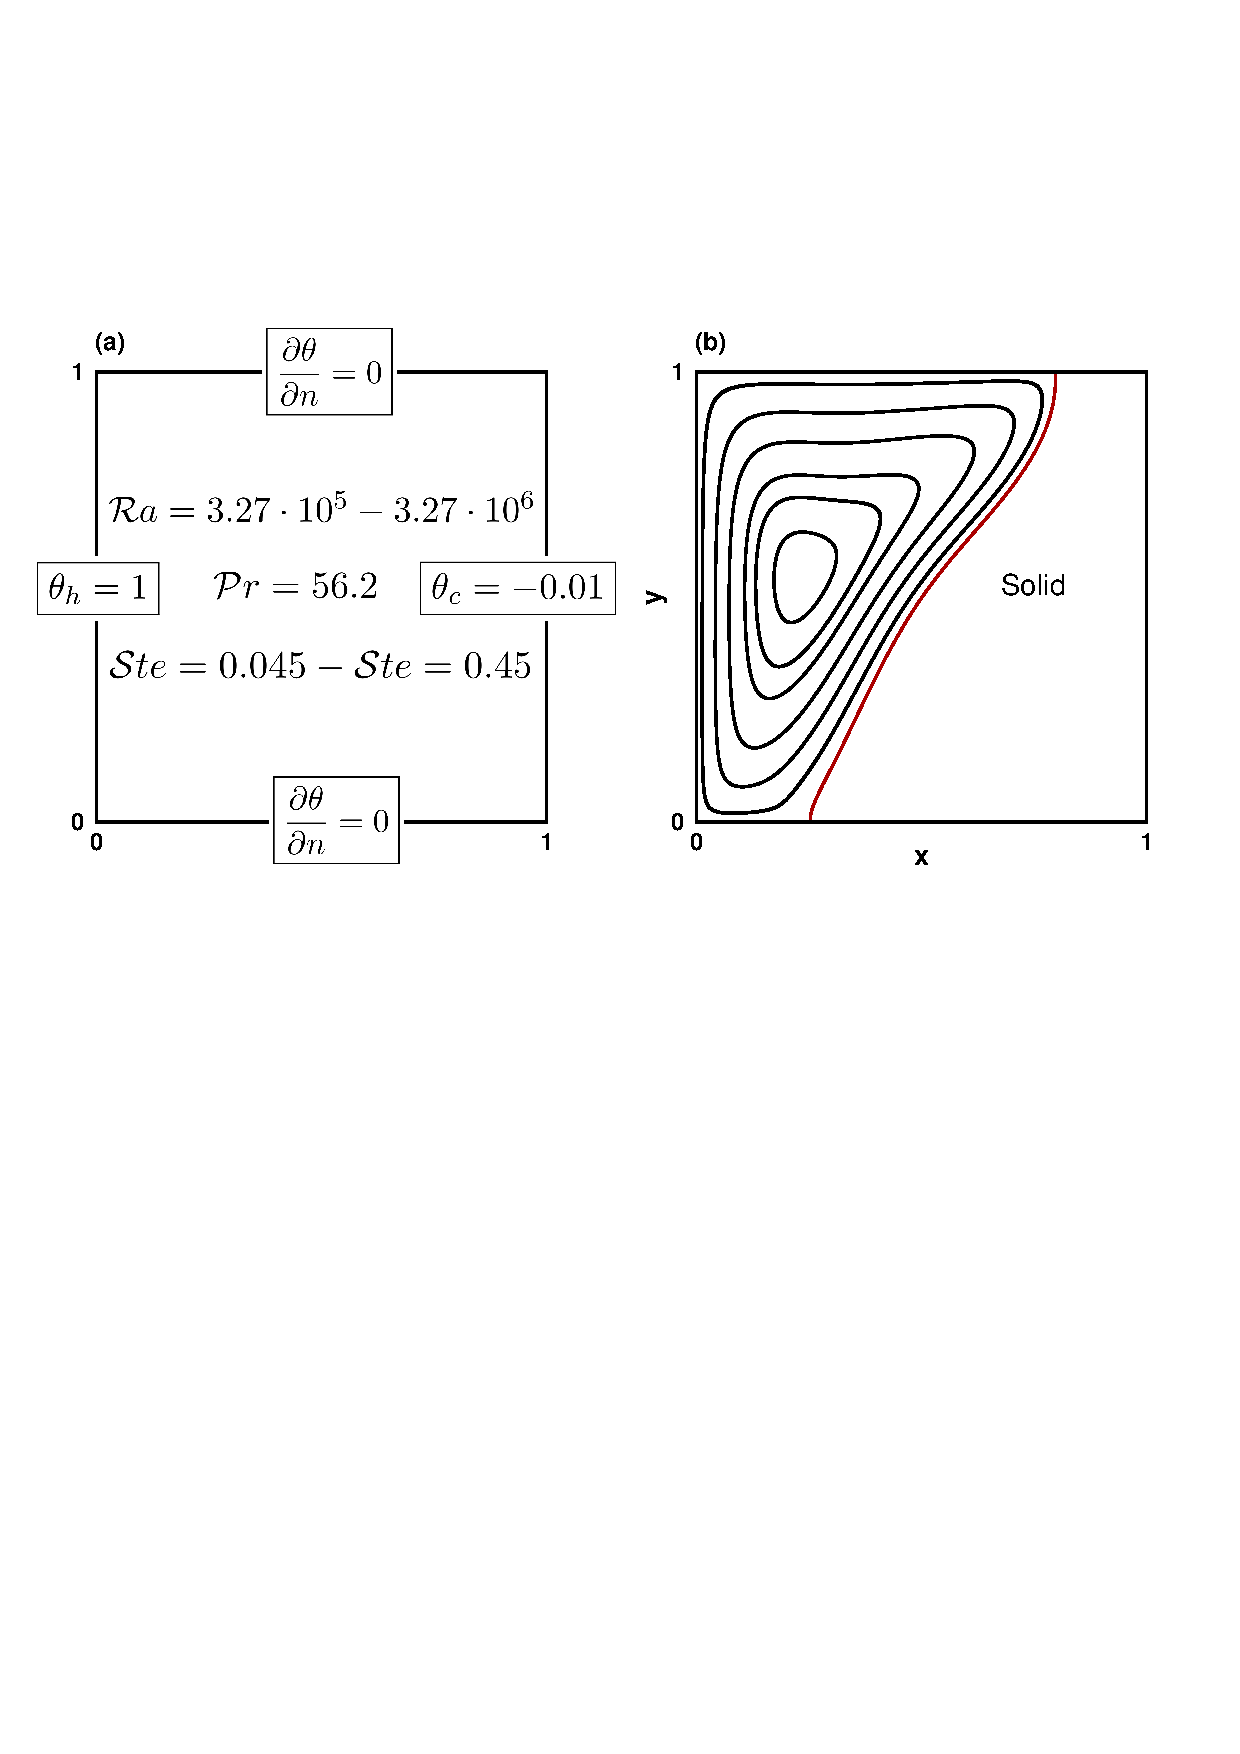
\includegraphics[width=.9\textwidth]{\figpath/Fig_cap_melting_basal/Scheme-melt-lat} \\
		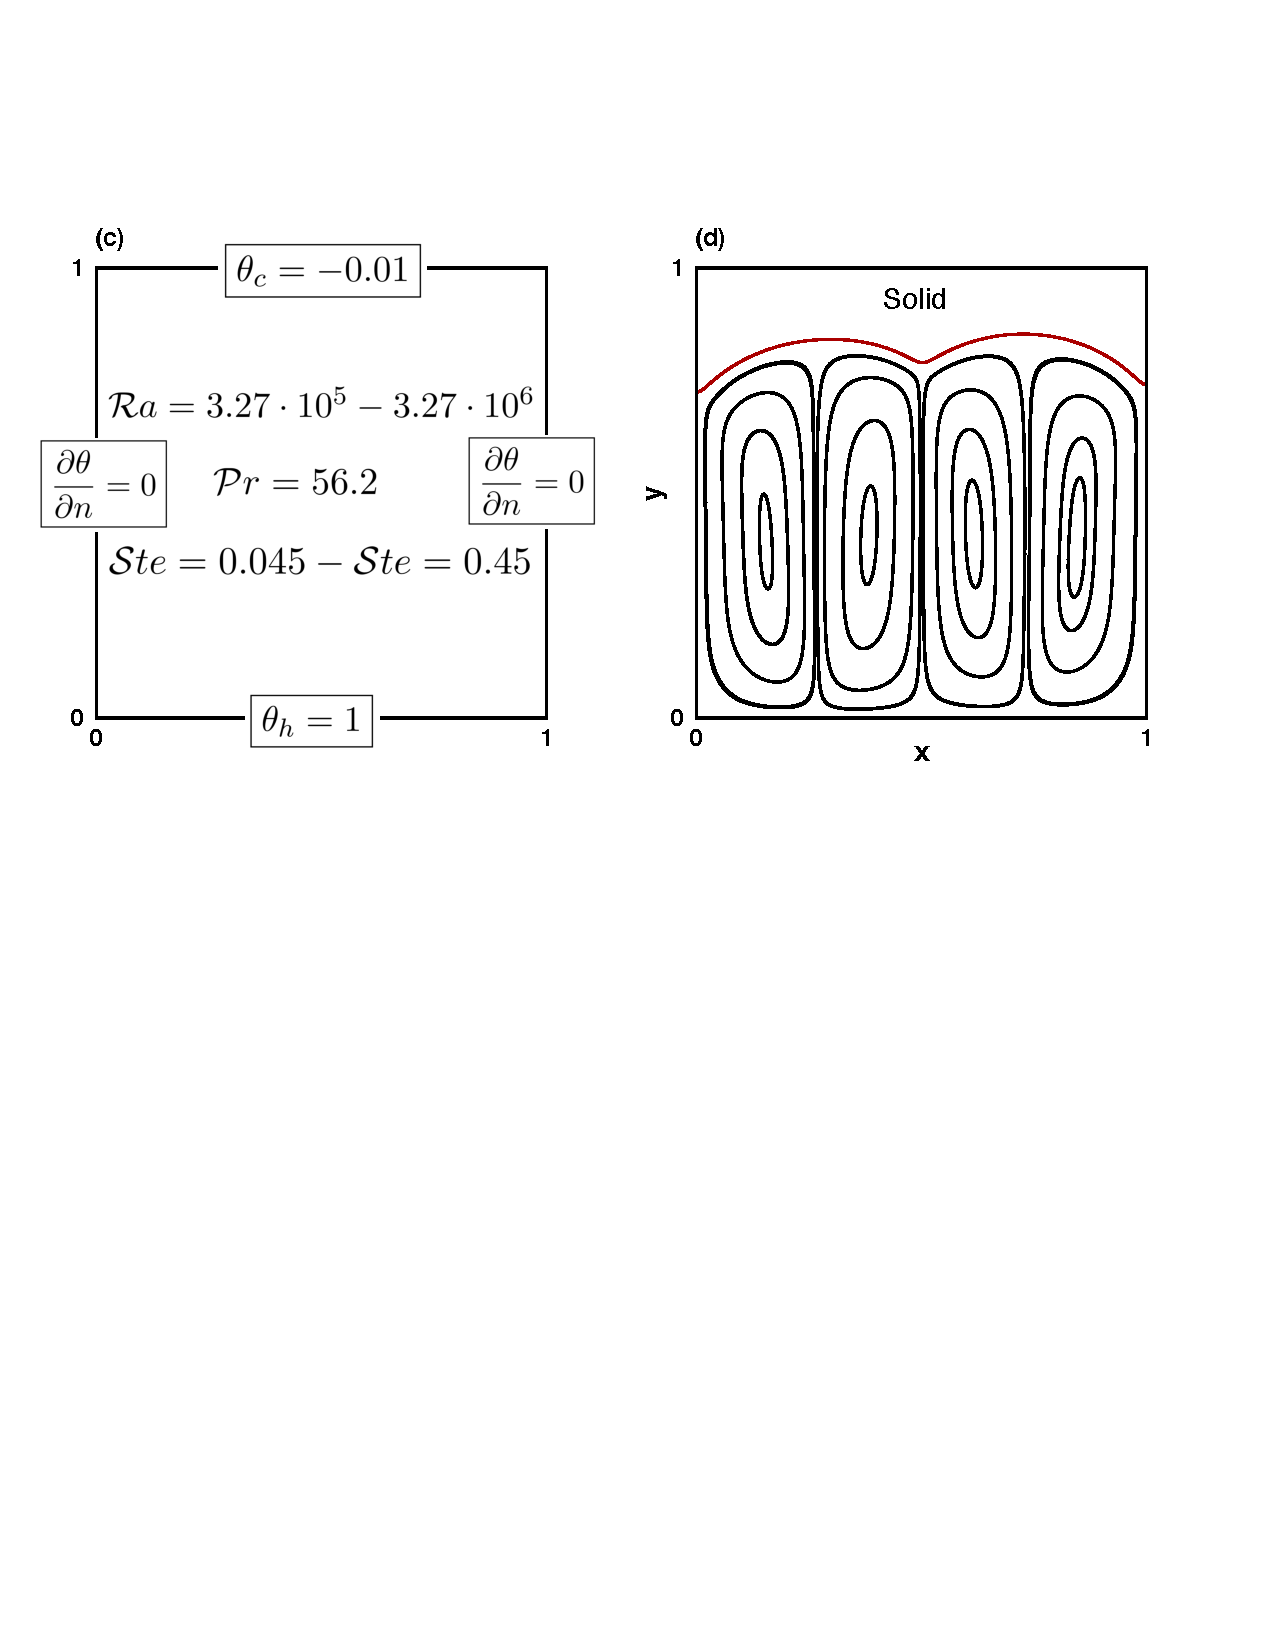
\includegraphics[width=.9\textwidth]{\figpath/Fig_cap_melting_basal/Scheme-melt-basal}
	\end{center}
	\caption{Sketch of the computational domain, boundary conditions for lateral (top) and basal (bottom) melting, streamlines showing the dynamic of the convection flow in the liquid phase (panels b and d) and solid-liquid interfaces (solid red lines).} \label{fig:melt-scheme}
\end{figure}
We have performed extensive validations of our numerical method in Chapters \ref{chap-NATCONV} and \ref{chap-MELTING}.
Very good agreements were noticed for all validation cases against well-known benchmarks and the robustness of the algorithm was proven by simulating challenging configurations.
We now use the code as an investigation tool to analyse the phase-change process during the melting stage.
We consider a square cavity of height $H$ filled with n-octadecane PCM and pay a closer attention to the temporal evolution of different physical parameter of the system. 

Two classes of convective melting systems are of interest in this chapter: \textbf{(i)} lateral melting (LM) or \textbf{(ii)}  basal melting (BM).
As far as \textit{(i)} is concerned, the PCM is subject to heating from the left side of the cavity, whereas for BM case the PCM is heated from the bottom within top melting boundary.
The comparison of both cases is appealing since the dynamic of the melting is known to be fundamentally different for each of the two cases.
The shape of the interface and the streamlines in the fully developed convective flow are illustrated in panels (b) and (d) of Fig. \ref{fig:melt-scheme} for both cases using the same physical parameters (see Figs. \ref{fig:melt-scheme}a and \ref{fig:melt-scheme}c).
LM case exhibits a mono cellular pattern while Rayleigh-B�nard-like convection cells are features of the BM case. 

\noindent LM case could be representative of building applications, at the example of the melting of a brick of PCM we simulated in Sec \ref{sec: melting-2D} of Chapter \ref{chap-MELTING},
in which a transparent brick of PCM is used as smart material to control the indoor environment of a building.
\cite{barreneche2016situ} have actually shown that wall made of PCMs allows to reduce the temperature peak about $20 \%$.
Bricks made of PCM melt from differences between outdoor and indoor temperatures and store the energy in the form of latent heat.
Other applications such as solar collectors or other thermal energy storages are also typical of such configurations.
In any cases, accurate assessment of the heat transfer is always essential.
Analytical investigation of \cite{bejan1989analysis} and scaling analysis of \cite{jany1988scaling} have permitted to describe the heat transfer during the melting by the mean of $\Nuss$-$\Ray$ correlation. 

\noindent The second class refers to passive temperature control for electronic devices or for a long list of geophysical problems,
such as lava lakes, thermal convection in magma chambers, or ice-melt lakes. 
%Ice-melt ponds that form during summer season in the Arctic \citep{polashenski2012mechanisms,esfahani2018basal} are known for example to display natural convection coupled to a phase-change process on the bottom side. In that case, Rayleigh-B�nard like convection cells are observed in the liquid phase.
Experimental and numerical investigations of the dynamic of the melting could be find in the literature for BM case.
However, in contrast with LM case,
notwithstanding linear and weakly non-linear instability analysis based on a vanishingly small Stefan number assumption \citep{vasil2011dynamic}, exact expression of $\Nuss$ and $L_f$ from purely theoretical work are not available during the convective regime due to the important non-linearities of the dynamics.
Some comparisons with theories \citep{malkus1954heat,grossmann2000scaling} made in the frame of Rayleigh-B�nard convection flow have been however carried out \citep{esfahani2018basal,madruga2018dynamic,favier2019rayleigh}.

%Numerical comparison of n-octadecane PCM with either lateral (LM) or basal melting (BM) is investigated in this chapter.
%Mainly a comparison of the heat transfer involving in each case is of major interest.
We analyse first the time evolution of the LM process through a scale analysis in Sec. \ref{sec-melting-lateral}.
Second, the BM case is performed in Sec. \ref{sec-melting-basal} with theoretical descriptions of the heat transfer involving during the melting.
Finally, a comparison between LM and BM cases is presented in Sec. \ref{sec-compare-LM-BM}.

\section{Lateral melting of n-octadecane PCM. Case LM}  \label{sec-melting-lateral}
We consider the physical properties of n-octadecane given in Tab. \ref{tab-param-PCM} and investigate
different height $H$ of the cavity and different value of $\delta T$, to assess the influence of the $\Ray$ number.
The numerical configuration is sketched in Fig. \ref{fig:melt-scheme}a.
$\Ray$ numbers ranging from $3.27 \cdot 10^5$ to $3.27 \cdot 10^6$ are investigated.
We note that for the range of $\Ray$ and $\Ste$ numbers of interest, the assumption of $(\beta \times \delta T) \ll 0.01$ is verified.

\noindent A second dimensionless time $\tau$ related to the analytical correlation of \cite{jany1988scaling} is introduced:
\begin{equation}
\label{eq-adim-tau}
\tau = \Ste\cdot \mathcal{F}o = \Ste\cdot \frac{\alpha t_{\varphi}}{H^2}  = \frac{\Ste}{\Prd} \cdot t,
\end{equation}
where $\mathcal{F}o$ is the Fourier number. 

\subsection{Analysis of the time evolution of the melting process} \label{subsec-time-evol-lat}

We start by describing the time evolution of the melting process for the lowest value of the Stefan number $\Ste = 0.045$.
We are interested in a slowly melting of the PCM to capture the transitions between the regimes described by \cite{jany1988scaling}, mainly the onset of the convective regime.

\noindent At $\tau=0$, the material is solid and the initial temperature is set to $\theta_0=-0.01$ everywhere inside the cavity. 
Then, the temperature of the left wall is progressively increased to $\theta_h=1$, while the right wall is maintained at the same cold temperature $\theta_c=-0.01$. 
The material starts to melt, with a melting front (identified by the iso-line $\theta=\theta_f=0$) propagating from the left to the right side of the domain. 
%The shape of the interface and the streamlines of the flow developing in the liquid phase when the convective flow is fully developped at $\tau = 0.06$ are illustrated in Fig. (\ref{fig:melt-scheme}b).
\begin{figure}
	\begin{center}
		%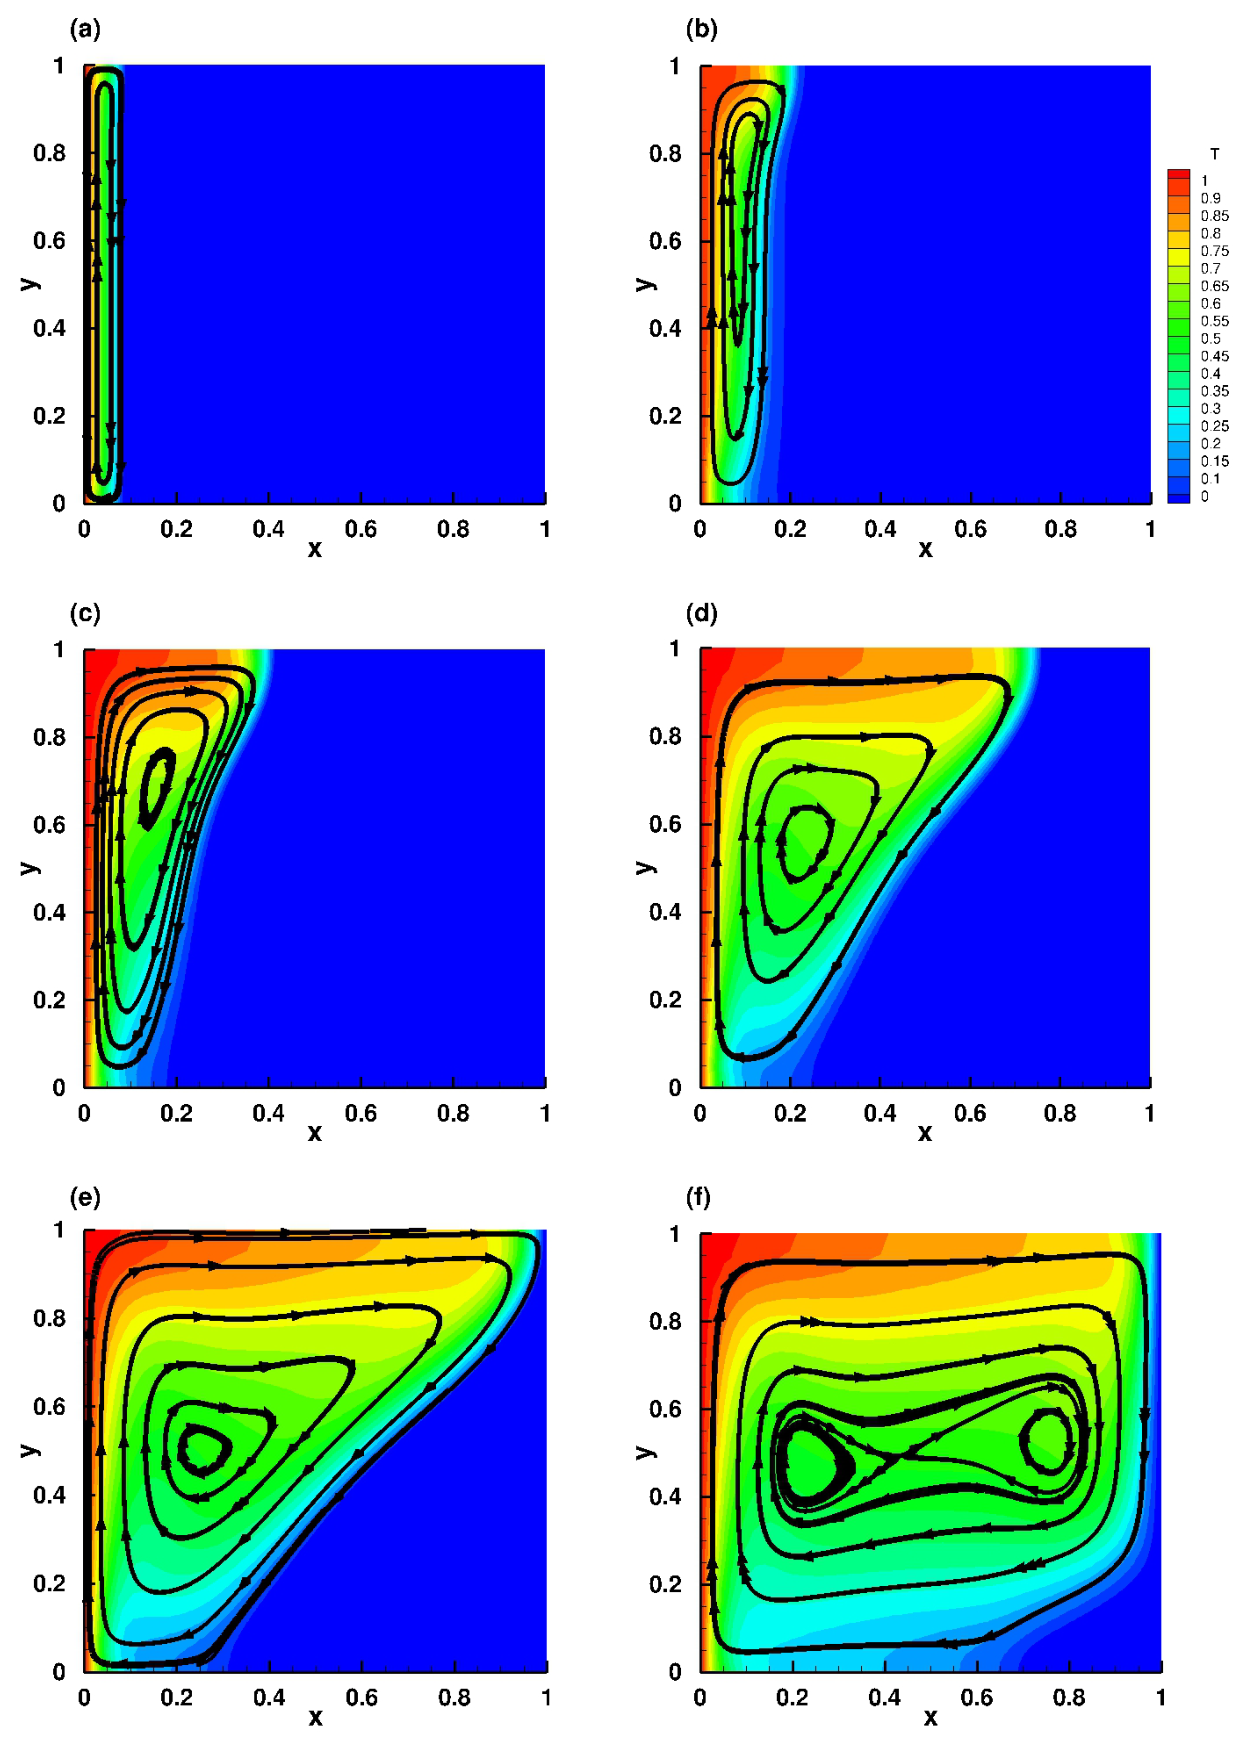
\includegraphics[width=.9\textwidth]{\figpath/Fig_cap_melting/fig05}
		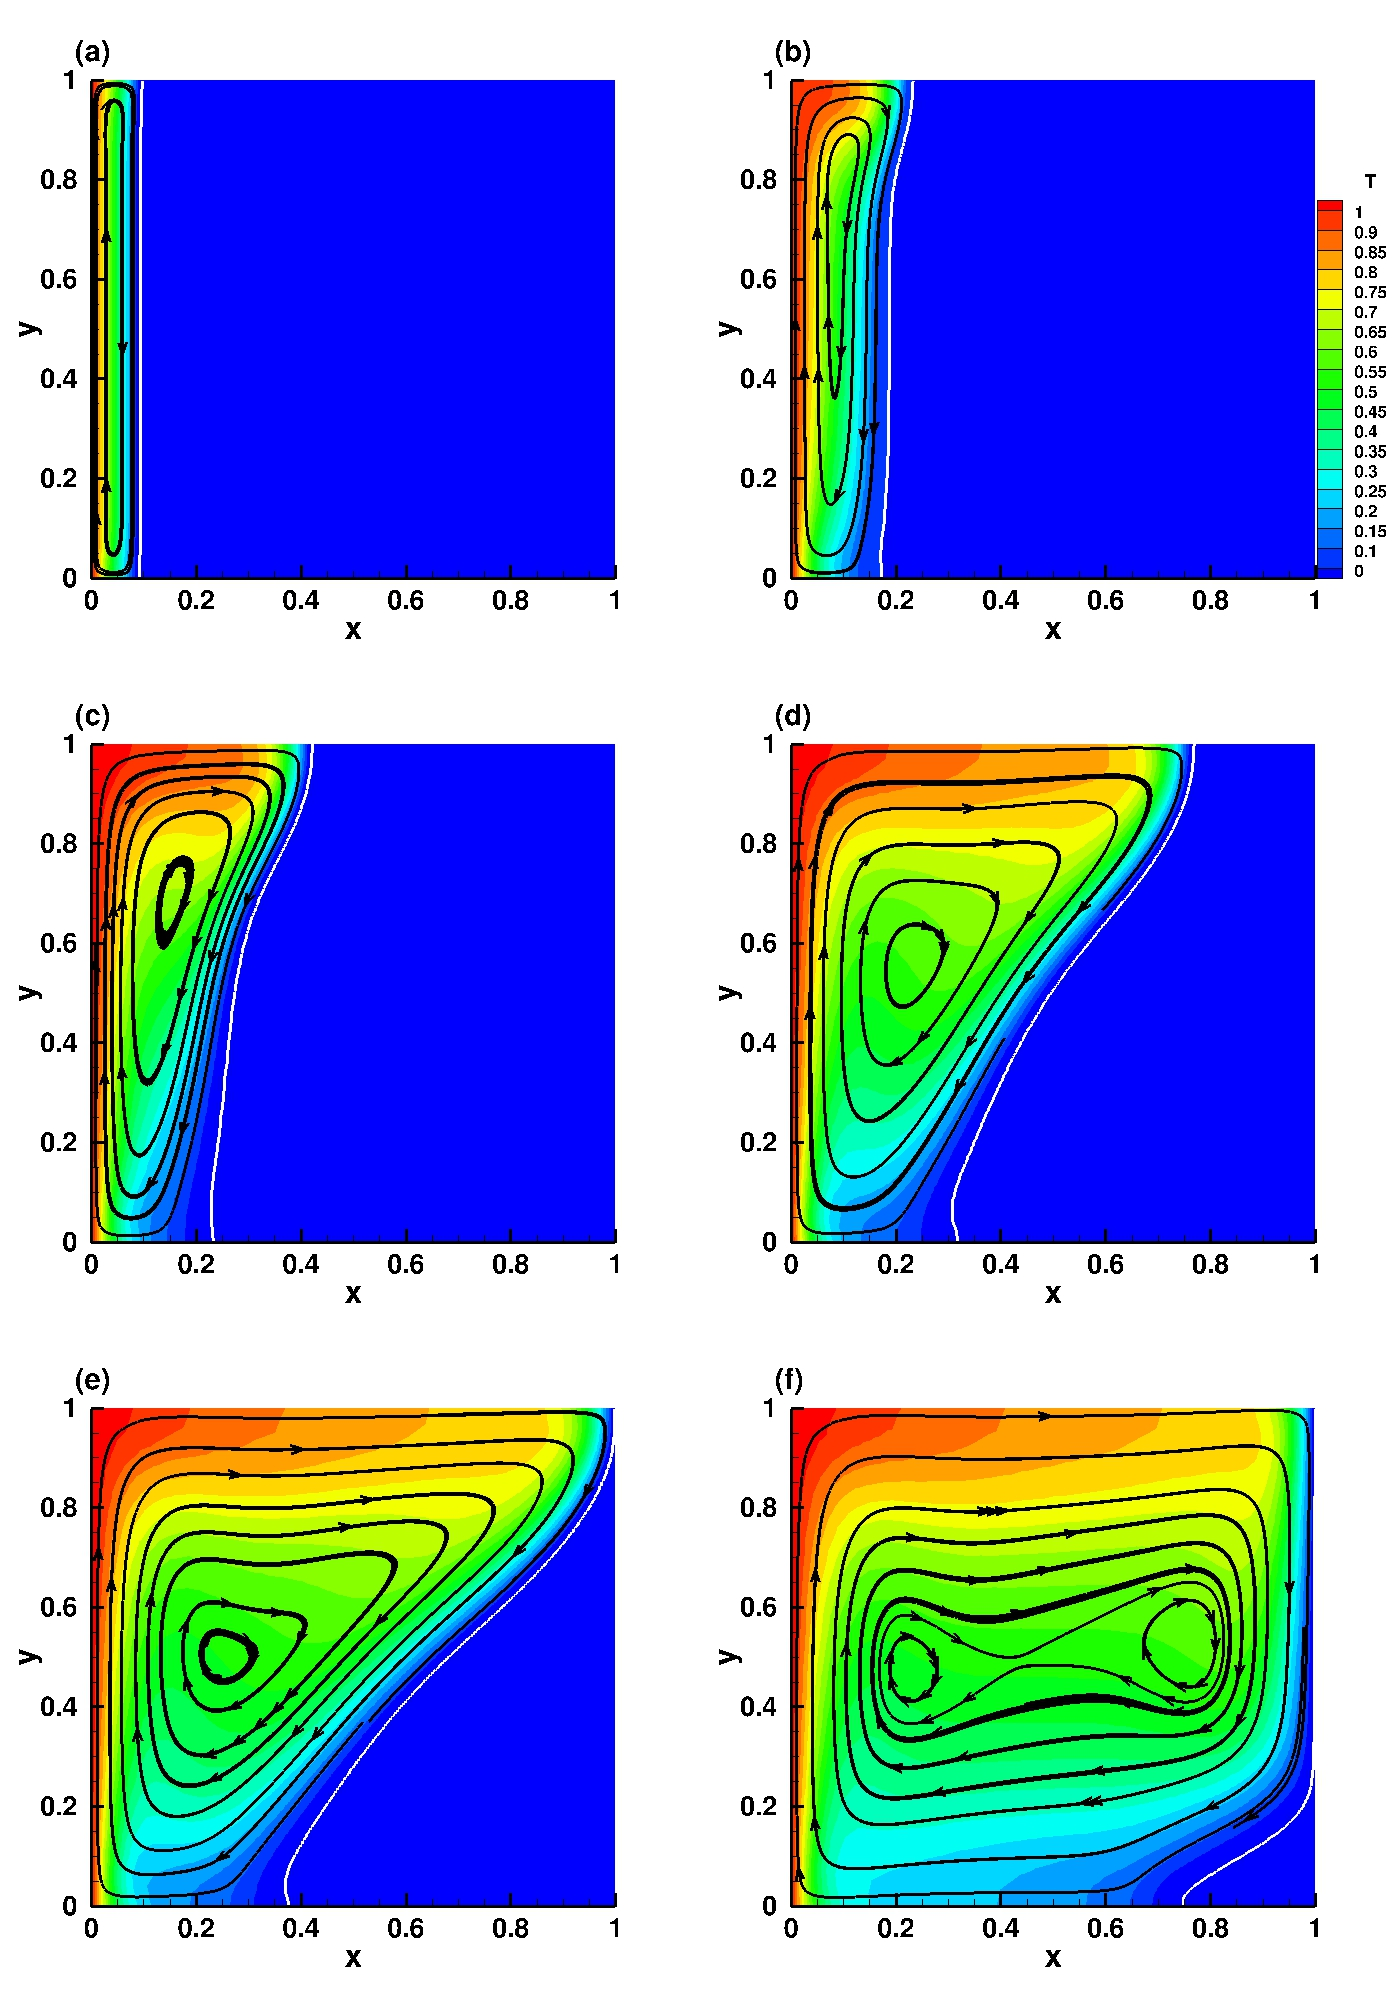
\includegraphics[width=.9\textwidth]{\figpath/Fig_cap_melting_basal/MELT_cavity_field}
	\end{center}
	\caption{Temperature iso-lines and streamlines in the fluid phase. The solid part is represented in blue and corresponds to the region of temperature $\theta \leq \theta_f=0$. Time instants (panels  a to f): $\tau=0.004; 0.016; 0.032; 0.063; 0.08; 0.2$. $\Ray = 3.27 \cdot 10^5$, $\Pr = 56.2$ and $\Ste = 0.045$.
		}\label{fig:melt-field}
\end{figure}

\noindent Snapshots of the time evolution of the phase-change system are given in Fig. \ref{fig:melt-field} for representative time instants.
Panels (a) to (f) offer the streamline showing the clockwise recirculation of the fluid, the melting front, and the temperature distribution (the solid phase is denoted by the blue region) for a comprehensive description of the evolution of the system. 
We can easily identify three different regimes describing the time evolution of the melting process. 
\begin{itemize}
	\item From $\tau=0$ to $\tau =0.004$ (Fig.  \ref{fig:melt-field}a), we note the vertical shape of the melting front, well predicted by the classical conduction model of \cite{stefan1891theorie}. This indicates that, at this stage, heat transfer is dominated solely by conduction.
	
	 \item Between $\tau =0.016$ to $\tau =0.032$ (Fig.  \ref{fig:melt-field}b), the natural convection in the fluid phase starts to alter the shape of the melting front.
	A mixed conduction and convection regimes rule the heat transfer. 	
	Convective flow mainly affects the upper part of the fluid motion, while conduction is still dominating in the lower part. As the volume thermal expansion coefficient $\beta$ is positive, we expect a clockwise circulation of the liquid inside the convection cell, as noted by \cite{jany1988scaling}.
	This also makes the liquid-solid interface to move faster at the top of the cavity, explaining the deformed shape of the melting front, which is a signature of the convection effects  (see also \cite{kowalewski2004phase}). 
	
	\item After $\tau=0.032$ (Fig.  \ref{fig:melt-field}c-d), natural convection dominates the heat transfer process and impacts radically the solid-liquid interface shape and motion.
	The melting front line exhibits four distinct regions characterized by different slopes with respect to the vertical axis. The largest slope is observed at the top of the cavity and is related to the particular shape of the convection cell. Note that top and bottom parts of the interface are normal to the cavity boundaries because of the imposed adiabatic boundary conditions.

	\item After $\tau =0.08$  the melting front is nearly touching the right wall of the cavity, firstly at the top (Fig.  \ref{fig:melt-field}e) of the cavity. The melting process continues and the fluid progressively fills the cavity, with a melting front  deforming to a vertical line. The  simulation of the melting process is stopped at $\tau =0.2$ (Fig.  \ref{fig:melt-field}f), when it is numerically difficult to separate the melting front from the right wall boundary. At this time instant,  the fluid fraction reaches the value of $0.95$ and  the melting of the PCM is considered to be complete, even though a small region of solid PCM remains at the lower right bottom of the cavity. Note from Fig.  \ref{fig:melt-field}f the existence in the fluid  of two recirculating zones instead of a single one observed during previous stages.
	
\end{itemize}

\subsection{Scale analysis of the melting} \label{sec:scaling anal}

We further analyse each of the three regimes cited previously and identify the proper scales of the phenomenon.
%The following analysis is similar to that outlined in Sec. \ref{sec-bound-scal-anal} for natural convection problem without phase-change.
The (dimensionless) location of the interface will be denoted by $\Gamma_i$.

Immediately after $t=0$ (see Fig. \ref{fig:melt-field}a), the melted PCM occupies a thin enclosure of height $H$ and width $\Gamma_i$.
In such configuration, the temperature varies linearly between the two sidewalls and the heat transfer is essentially ruled by conduction. 
The fluid phase is almost motionless and the horizontal heat flux across the incipient melting PCM is balanced by the enthalpy absorbed at the interface.
At the solid-liquid interface, the energy balance condition which takes into account the released latent heat and the discontinuity of heat flux between the solid and the liquid can be handle by the following Stefan condition:
%\begin{eqnarray} \label{eq:Ste-condition}
%	\left. T\right|_{x=\Gamma_i} &=& T_f, \\ \nonumber
%	\rho h_{sl} \frac{\partial \Gamma_i}{\partial t_{\varphi}} &=& - k \frac{\partial T}{\partial n},
%\end{eqnarray}
\begin{eqnarray} \label{eq:Ste-condition}
	\theta (x=\Gamma_i) &=& \theta_f =  0, \\ \nonumber
	\frac{\partial \Gamma_i}{\partial t} &=& - \frac{\Ste}{\Prd} \frac{\partial \theta}{\partial x},
\end{eqnarray}

%, with $\Gamma_i \ll H$ (and thus $\partial^2 \theta/\partial y^2 \ll \partial^2 \theta/\partial x^2$).


%Accordingly, the interface remain vertical during this stage.
%Since the velocity in the liquid phase is relatively small during this conductive regime, the momentum, the energy equation, and the Stefan condition at the interface could be rewritten in the small enclosure containing the melted PCM as
%\begin{eqnarray} \label{eq-balance-momentum}
%   \frac{\partial p}{\partial x} &=& \frac{\Ray}{\Rey^2 \Prd} \theta, \\ \label{eq-energy-x}
%    \frac{\partial \theta}{\partial t} &=& \frac{1}{\Rey \Prd} \frac{\partial^2 \theta}{\partial x^2}, \\ \label{eq-stefan-x}
%   \frac{\partial \Gamma_i}{\partial t} &=& - \frac{\Ste}{\Prd} \frac{\partial \theta}{\partial x}.
%\end{eqnarray}

\noindent Since the temperature field during the conduction regime is quasi-steady, the linear Eq. \ref{eq:Ste-condition} could be approximated by
\begin{equation}
    \frac{\partial \Gamma_i}{\partial t} \approx - \frac{\Ste}{\Prd} \frac{\theta_f - \theta_h}{\Gamma_i} \approx  \frac{\Ste}{\Prd} \frac{1}{\Gamma_i}.
\end{equation}

\noindent The location $\Gamma_i$ of the interface is consequently given by
\begin{equation} \label{eq-cond-evol}
   \Gamma_i = \sqrt{2 \times \frac{\Ste}{\Prd} t} = \sqrt{2 \tau}.
\end{equation}

\noindent Moreover, the Nusselt number can be evaluated using the same assumption,
\begin{equation}
   \Nuss= \int_0^{1} \left. \frac{\partial \theta}{\partial x} \right|_{x=0} dy = \frac{1}{\Gamma_i} = ({2 \tau})^{-1/2}.
\end{equation}

\noindent To summarize, during the first stage of the melting, when the heat transfer is led by conduction, the time evolution of the liquid fraction (given by the location of the interface) and the Nusselt number could be approximated by
\begin{eqnarray} \label{eq-Nu-Lf-Corr-Lat}
	L_f &\sim& (2 \tau)^{1/2}, \\ 
	\Nuss &\sim& (2 \tau)^{-1/2}.
\end{eqnarray}

\begin{figure}
	\begin{center}
		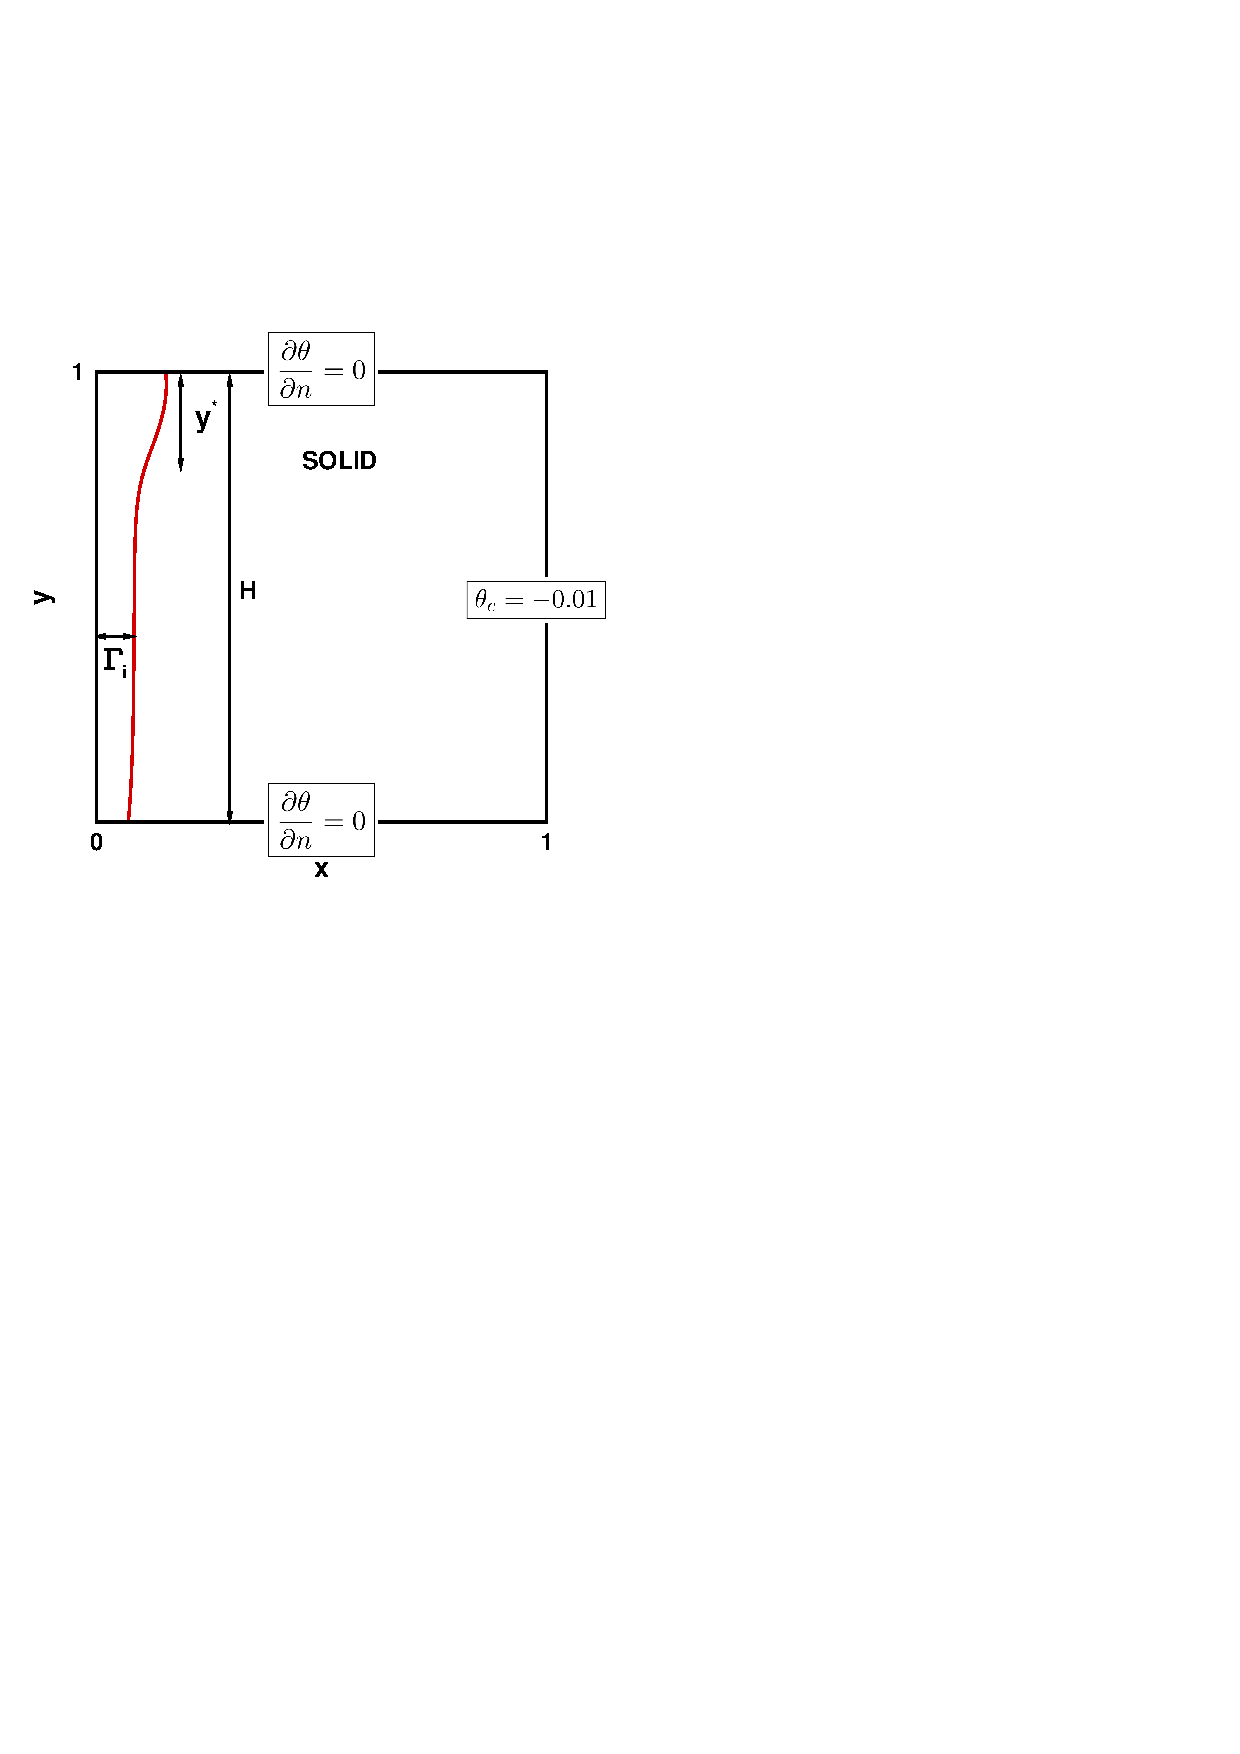
\includegraphics[width=.5\textwidth]{\figpath/Fig_cap_melting_basal/MELT_Regime_evol}
	\end{center}
	\caption{Illustration of the mixed regime. Solid red line is the solid-liquid interface, $\Gamma_i$ represents the location of the interface and $y^*$ denotes the height of fluid impacted by the emerging convective flow.}\label{fig:melt-scheme-regime}
\end{figure}

While the melting continues to expand to the right side of the domain, a natural convection flow emerges from the top of the cavity (see Fig. \ref{fig:melt-scheme-regime}).
Convection and conduction coexist at this stage and
the total heat transfer rate is thus the sum of the conductive and the convective heat transfer.
Turning back to the energy Eq. \ref{eq-energ} in the liquid phase  (i.e. $C = K = 1$), three distinct effects could be identified:
\begin{equation}
	\underbrace{\frac{\delta \theta}{t}}_{Inertia} \quad \underbrace{v \frac{\delta \theta}{H}}_{Convection} \quad \underbrace{\frac{\delta \theta}{\Gamma_i^2}}_{Conduction},
\end{equation}

\noindent As $t$ increases, the inertia decreases in importance while the convection effect increases since it is proportional to $v$, and the conduction becomes more and more negligible with the increasing value of $\Gamma_i$ with time. 
To assess for the convective heat transfer contribution during this mixed regime,
one can define a Rayleigh number based on $y^*$ as $\Ray_{y^*} = \Ray \times y^{*3}$,
with $y^{*}$ the height of the melted zone altered by the convection flow as shown in Fig. \ref{fig:melt-scheme-regime} (see also  \cite{jany1988scaling}).
We note that at the bottom part of the cavity, the interface remains vertical by the effect of the conductive heat transfer.
Since $\Pr \gg 1$, the scaling presented in Eq. \ref{eq-scale-nbd-high-Pr} allows to evaluate the thickness of the thermal boundary layer in the top region as
 \begin{equation} \label{eq-conv-cond-reg}
 \delta_{\theta}^* \sim y^* \times \Ray_{y^*} ^{-1/4}.
\end{equation}

\noindent A this stage, the thickness $\delta_{\theta}^*$ of the thermal boundary layer is proportional to the thickness of the liquid zone $\Gamma_i$ ($\sim \sqrt{2 \tau}$) resulting that
 \begin{equation}
	 y^* \sim (2 \tau)^2 \times \Ray. %\quad  \Rightarrow \quad \frac{y^*}{\Gamma_i} \sim (2 \tau)^{3/2} \times \Ray.
 \end{equation}
 
 \noindent The Nusselt number related to this region is hence
  \begin{equation}
   \Nuss= \int_{1-y^*}^{1} \left. \frac{\partial \theta}{\partial x} \right|_{x=0} dy = \frac{y^*}{\Gamma_i} \sim (2 \tau)^{3/2} \times \Ray.
\end{equation}

\noindent The total Nusselt number during the mixed convection-convection regime can therefore be approximated by
\begin{equation} \label{eq-Nu-conv-cond}
   \Nuss \sim (2 \tau)^{-1/2} + (2 \tau)^{3/2} \times \Ray.
\end{equation}

\noindent Eq. \ref{eq-Nu-conv-cond} indicates that the contribution of the conduction $\left(\sim 1/\sqrt{2 \tau}\right)$ decreases with the time while the convection one is increasing.
%From a simple analysis of $\partial \Nuss/\partial \theta = 0$, one can find the minimum value of the Nusselt number $\Nuss_{min} \sim Ra^{1/4}$ occurring at $\tau \sim \Ray^{-1/2}$.

Finally, when the natural convection flow is fully developed and dominates the heat transfer along the vertical heated wall, the dimensionless thickness of thermal boundary layer is $\delta_{\theta} \sim \Ray^{1/4}$ and therefore the Nusselt number scale is
\begin{equation} \label{eq-Nu-Ra-LM}
   \Nuss \sim \Ray^{1/4}
\end{equation}

\cite{Okada1984} have suggested from his experimental data the following correlation of $\Nuss$ taking into account the foregoing presented regimes:
\begin{equation} \label{eq-corr-Okada}
	\Nuss = \left \{
	      %\begin{array}{ll}
	      \begin{aligned}
	      		\frac{1}{\sqrt{2 \tau}} \quad  &\text{if} \quad \tau \leq \tau_t, \\ 
	      		\frac{1}{\sqrt{2 \tau_t}} \left \{ 1 + C (\tau - \tau_t) \right \} \quad & \text{if} \quad \tau > \tau_t, \\
			c_1 \Ray^{0.266} \quad & \text{otherwise},
	       %\end{array}  
	       \end{aligned}
	\right.
\end{equation}
with the constant $c_1 = 0.234$ and the power $0.266$ fitted from the experimental data, and $\tau_t$ the transition time from conduction to convection as discussed previously.

\noindent \cite{jany1988scaling} have proposed more general single correlation, also combining the regimes described previously:
\begin{equation} \label{eq-Nu-scale}
\Nuss(\tau) =  \frac{1}{\sqrt{2 \tau}} + \left[c_1 \Ray^{1/4} - \frac{1}{\sqrt{2 \tau}} \right]  \left[ 1 + \left(c_2 \Ray^{3/4}  \tau^{3/2}\right)^n \right]^{1/n}.
\end{equation}
The values of the constants were fitted from numerical data: $c_1 = 0.27$, $c_2 = 0.0275$, and $n=-2$. 

\noindent Both of Eqs. \ref{eq-corr-Okada} and \ref{eq-Nu-scale} are compared with our numerical results in Fig. \ref{fig:Nusselt} showing the time evolution of the Nusselt number at the left wall.
Our results perfectly fit with the theoretical prediction of \cite{jany1988scaling} and are also in good agreement with the correlation of \cite{Okada1984}. 
The gap between the current simulation and the results of \cite{Okada1984} could be explained by the experimental heat loss mentioned by the author and the uncertainties of the experimental measurements.
The regimes described by the shape of the interface in Sec. \ref{subsec-time-evol-lat} could be featured by the temporal evolution of $\Nuss$:
\begin{enumerate}
	\item The pure conduction regime ($\Nuss \sim (2 \tau)^{-1/2}$) for $\tau  \gtrsim 0$ to $\tau \sim \Ray^{-1/2} =0.02$  (corresponding to Fig.  \ref{fig:melt-field}a).
	Since the temperature gradient has initially huge values because of the increase of the temperature of the left wall, the Nusselt number rapidly decreases during the first stage of the flow evolution. 
	The  signature of this conduction regime is the slow heat transfer characterized by a monotonic decrease of the Nusselt number.
	
	\item The mixed conduction-convection regime  ($ \Nuss \sim \tau^{-1/2} + \Ray\, \tau^{3/2}$) for $  0.02  \leq \tau \leq 0.05$ (illustrated in  Fig.  \ref{fig:melt-field}b).

	\item The convection dominated regime ($ \Nuss \sim \Ray^{1/4}$) for $\tau > Ra^{-1/2}$  (corresponding to Figs.  \ref{fig:melt-field}c-e).
	The plateau at the value of $\Ray^{1/4}$ corresponds to the pure convective transfer and is observed in Fig. \ref{fig:Nusselt} for $  0.05 \leq \tau \leq 0.1$. Numerical results show a slight decrease of the $\Nuss$ in the final stage ($\tau \geq 0.1$), when the melting front starts to touch the right wall of the cavity (see Figs.  \ref{fig:melt-field}e-f). The correlation model is not valid for this late evolution of the melting process.
\end{enumerate}

\begin{figure}
	\begin{center}
		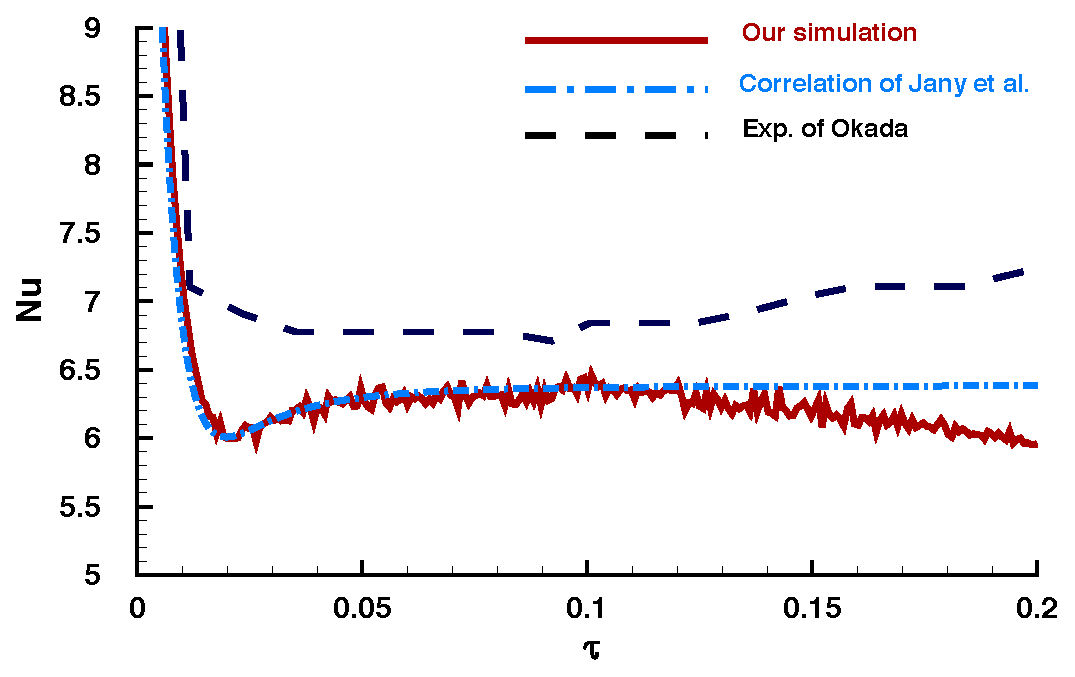
\includegraphics[width=.7\textwidth]{\figpath/Fig_cap_melting/fig06}		
	\end{center}
	\caption{Complete melting of the PCM. Time evolution of the average Nusselt number defined at the hot (left) wall (cf. Eq. \ref{eq-def-Nu}) (solid line). Comparison with the experimental results of  \cite{Okada1984} (dashed line) and the predictions using the correlation in Eq. \ref{eq-Nu-scale} suggested by \cite{jany1988scaling} (dash-dot line). $\Ray = 3.27 \cdot 10^5$, $\Pr = 56.2$ and $\Ste = 0.045$.}\label{fig:Nusselt}
\end{figure}


Another important basic quantity describing the melting process is the liquid fraction $L_f$.  
The time evolution of the liquid fraction (Fig. \ref{fig:Lf}a) displays three regimes during the melting process. $L_f$  initially grows as $\tau^{ 1/2}$, which is a typical law for a conduction-dominated heat transfer. Then, a linear temporal evolution is observed, until the melting front reaches the right wall.
This linear regime corresponds to the quasi-steady state observed in the evolution of the Nusselt number (Fig. \ref{fig:Nusselt}).

\noindent Using the asymptotic limits of Eq. \ref{eq-Nu-scale} for $ \tau \to 0$ (pure conduction) and $ \tau \to \infty$ (pure convection),  \cite{jany1988scaling} suggested the following correlation law for the time evolution of the liquid fraction:
\begin{equation} \label{eq-Lf-scale}
L_f(\tau) = \left[\left({\sqrt{2 \tau}} \right)^5 + \left(c_1 \Ray^{1/4}  \tau \right)^{5} \right]^{1/5},
\end{equation}
where $c_1=0.27$ is the same constant as in Eq. \ref{eq-Nu-scale}. 
We compare in Fig. \ref{fig:Lf}b our numerical results with the predictions based on Eq. \ref{eq-Lf-scale} within the validity domain of the analysis, \ie before the melting front reaches the right wall of the cavity. A very good agreement is found with theoretical predictions and also with previously published numerical results \citep{Wang2010}.

\begin{figure}[!ht]
	\begin{center}
		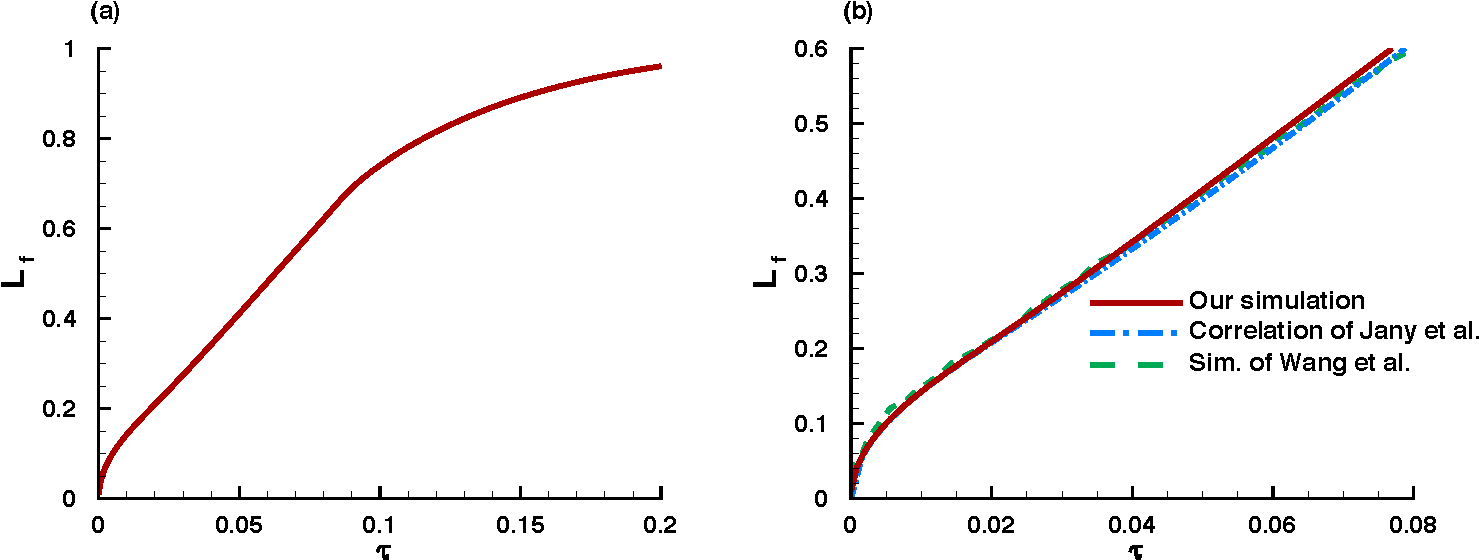
\includegraphics[width=0.9\textwidth]{\figpath/Fig_cap_melting/fig07}
	\end{center}
	\caption{Complete melting of the PCM. (a) Time evolution of the liquid fraction for the complete melting of the PCM. (b) Comparison of our results (solid line) with the numerical results of  \cite{Wang2010} (dashed line) and the predictions using the correlation (\ref{eq-Lf-scale}) suggested by \cite{jany1988scaling} (dash-dot line).}\label{fig:Lf}
\end{figure}


%%%%%%%%%%%%%%%%%%%%%ù
\subsection{Influence of the Rayleigh number}
%%%%%%%%%%%%%%%%%%%%%

\begin{figure}
	\begin{center}
		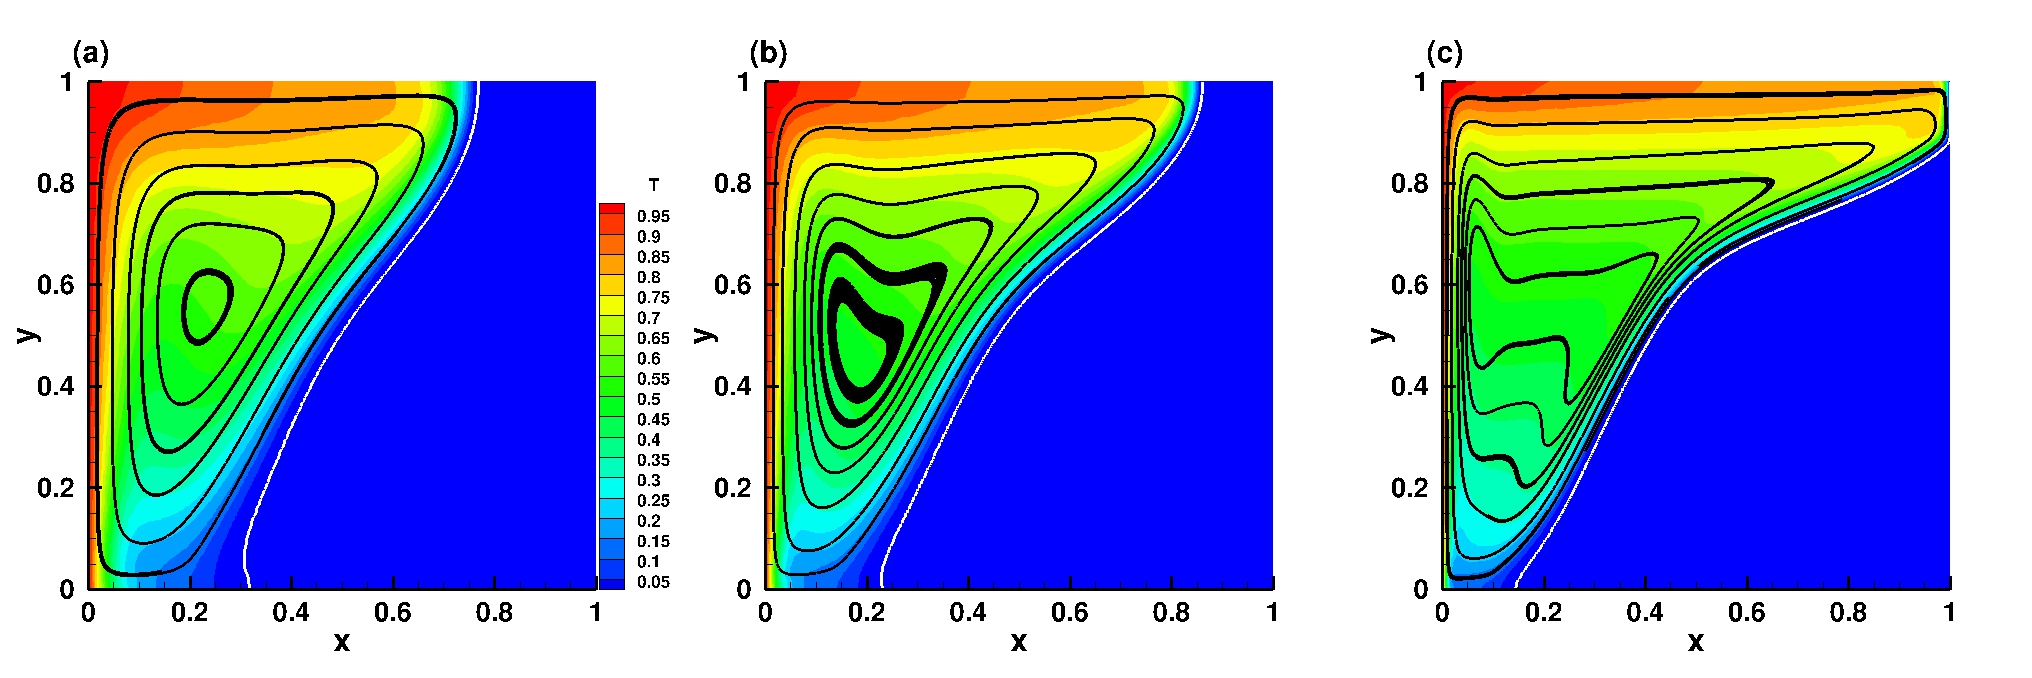
\includegraphics[width=\textwidth]{\figpath/Fig_cap_melting_basal/MELT_cavity_Ra_comp}
	\end{center}
	\caption{PCM melting at $L_f = 0.5$. Illustration of the temperature field, the streamlines, and the melting front for three $\Ray$ numbers: (a) $\Ray = 3.27 \cdot 10^5$ , (b) $\Ray = 1.62 \cdot 10^6$, (c) $\Ray = 3.27 \cdot 10^6$.
	The $\Prd$ and $\Ste$ numbers are kept constant: $\Prd = 56.2$ and $\Ste = 0.045$.} \label{fig:melt-comp-Ra}
\end{figure}

To investigate the influence of the Rayleigh number on the evolution of the melting process, we performed different simulations by multiplying the initial value of $\Ray = 3.27 \cdot 10^5$ by a factor of 5 and 10, respectively. The exact values are: $\Ray = 1.62 \cdot 10^6$ and $\Ray = 3.27 \cdot 10^6$. 
First, we increase the height $H$ of the cavity by a factor of $\sqrt[3]{5}$ and $\sqrt[3]{10}$ and consider the same $\delta T$.
Thus the $\Ste$ number is kept constant.
Second, we increase the temperature difference parameter $\delta T$ by keeping $H$ constant.
It corresponds of an increased value of the Stefan number by a factor of $5 $ and $10$:
$\Ste = 0.223$ and $\Ste = 0.45$.

Snapshots of numerical solutions for $\Ray = 3.27 \cdot 10^5$,  $\Ray = 1.62 \cdot 10^6$ and  $\Ray = 3.27 \cdot 10^6$ at constant $\Ste$ number are given in Fig. \ref{fig:melt-comp-Ra}.
The colours correspond to the temperature distribution, the  black lines correspond to the streamlines and the white lines correspond to the solid-liquid interface.
Panels (a) to (c) denote the dynamic of the convective melting when half of the initial solid PCM ($L_f = 0.5$) have melted.
The top part of the interface moves faster while the bottom one is slowed by the increasing value of $\Ray$.
According to the Stefan interface condition in Eq. \ref{eq-stefan-x}, at constant $\Ste$ and $\Prd$ numbers, the interface velocity is proportional to $\partial \theta / \partial n$, which is maximum at the top of the cavity because of the clockwise recirculation of the fluid explaining the observed trends.

Figs \ref{fig:Ra-Nusselt-H} and \ref{fig:Ra-Nusselt-deltaT} show the temporal evolution of the liquid fraction $L_f$ (panel a),  and the average Nusselt number defined at the hot wall (panel b). 
The same heat transfer regimes described previously are observed for each case: conduction, mixed conduction-convection and convection.
We note that results are plotted with respect to physical time $t_{\varphi}$ instead of $\tau$, 
because we compare solutions with different values of $H$, which involves in the definition of the non-dimensional times $t$ and $\tau$, making them not relevant to compare results.

\noindent Fig. \ref{fig:Ra-Nusselt-H}a indicates that increasing the Rayleigh number by keeping $\delta T$ constant induces a slower melting rate.
This is the expected behaviour since the size of the PCM is increased by a factor of 2, and the velocity $\vec u$ is decreasing to satisfy the condition $\Rey = 1$.
We note however a non-monotonic variation of the time necessary to melt a fixed value of fluid.
For instance, to achieve $L_f = 0.5$ (50\% of the volume is melted), an increase of $\Ray$ by a factor of $10$ leads to a growth of the time by a factor of $1.7$.
Nonetheless, when $\Ray$ is  $5$ times larger, the necessary time only increases by a factory of $2$.
This is most likely due to the non-linear intricacies of the problem and requires further investigation.\\
Furthermore, the Nusselt number reported in Fig. \ref{fig:Ra-Nusselt-H}b shows that the higher the Rayleigh number, the higher the Nusselt number.
This is consistent, since the temperature gradient is integrated along a greater heated wall. 

\noindent Fig. \ref{fig:Ra-Nusselt-deltaT}a shows that by increasing the value of $\delta T$, and consequently increasing the Rayleigh number and the Stefan number, the PCM melts faster. 
We note that the height $H$ of the cavity is kept constant, hence the natural convection flow in the melted PCM is enhanced when the Rayleigh number keep increasing.
As a consequence, the convection-dominated regime is reached earlier, as shown by the shift of the minimum of the $\Nuss$ to lower values of $t_{\varphi}$ in Fig. \ref{fig:Ra-Nusselt-deltaT}b. 
This evolution is also observed for the liquid fraction. 
As expected, an increase of the Rayleigh number and the Stefan number is followed by an enhancement of the heat transfer during the melting, and consequently an improved efficiency of the PCM.
\begin{figure}
	\begin{center}
		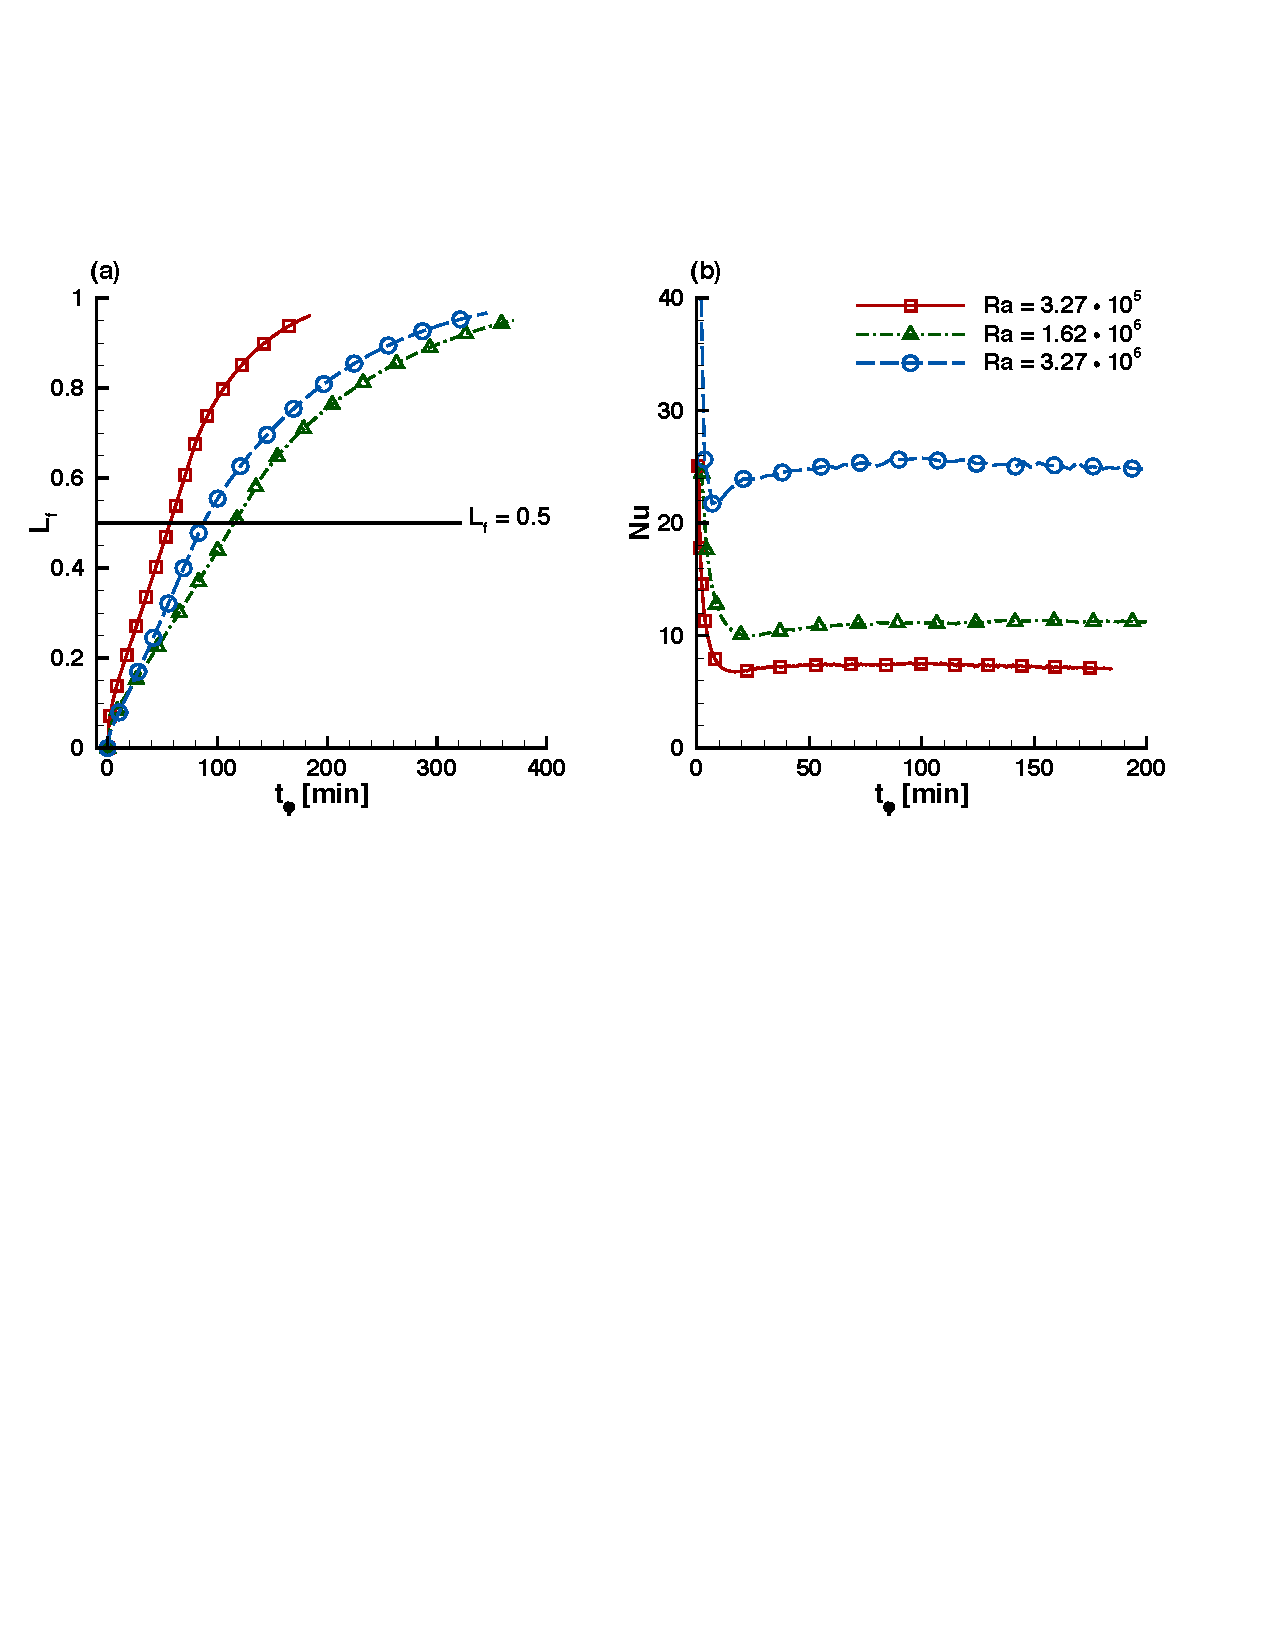
\includegraphics[width=.9\textwidth]{\figpath/Fig_cap_melting/fig08_2}
	\end{center}
	\caption{Complete melting of the PCM.  Influence of the value of the Rayleigh number ($\Ray$) on the time evolution of the liquid fraction (a) and the average Nusselt number defined at the hot (left) wall (b). The reference case ($\Ray=3.27\cdot 10^5$) is represented by red continuous lines. The value of the $\Ray$ was increased by a factor of $5$ and $10$, respectively while the Stefan number $\Ste$ is kept constant.}\label{fig:Ra-Nusselt-H}
\end{figure}

\begin{figure}
	\begin{center}
		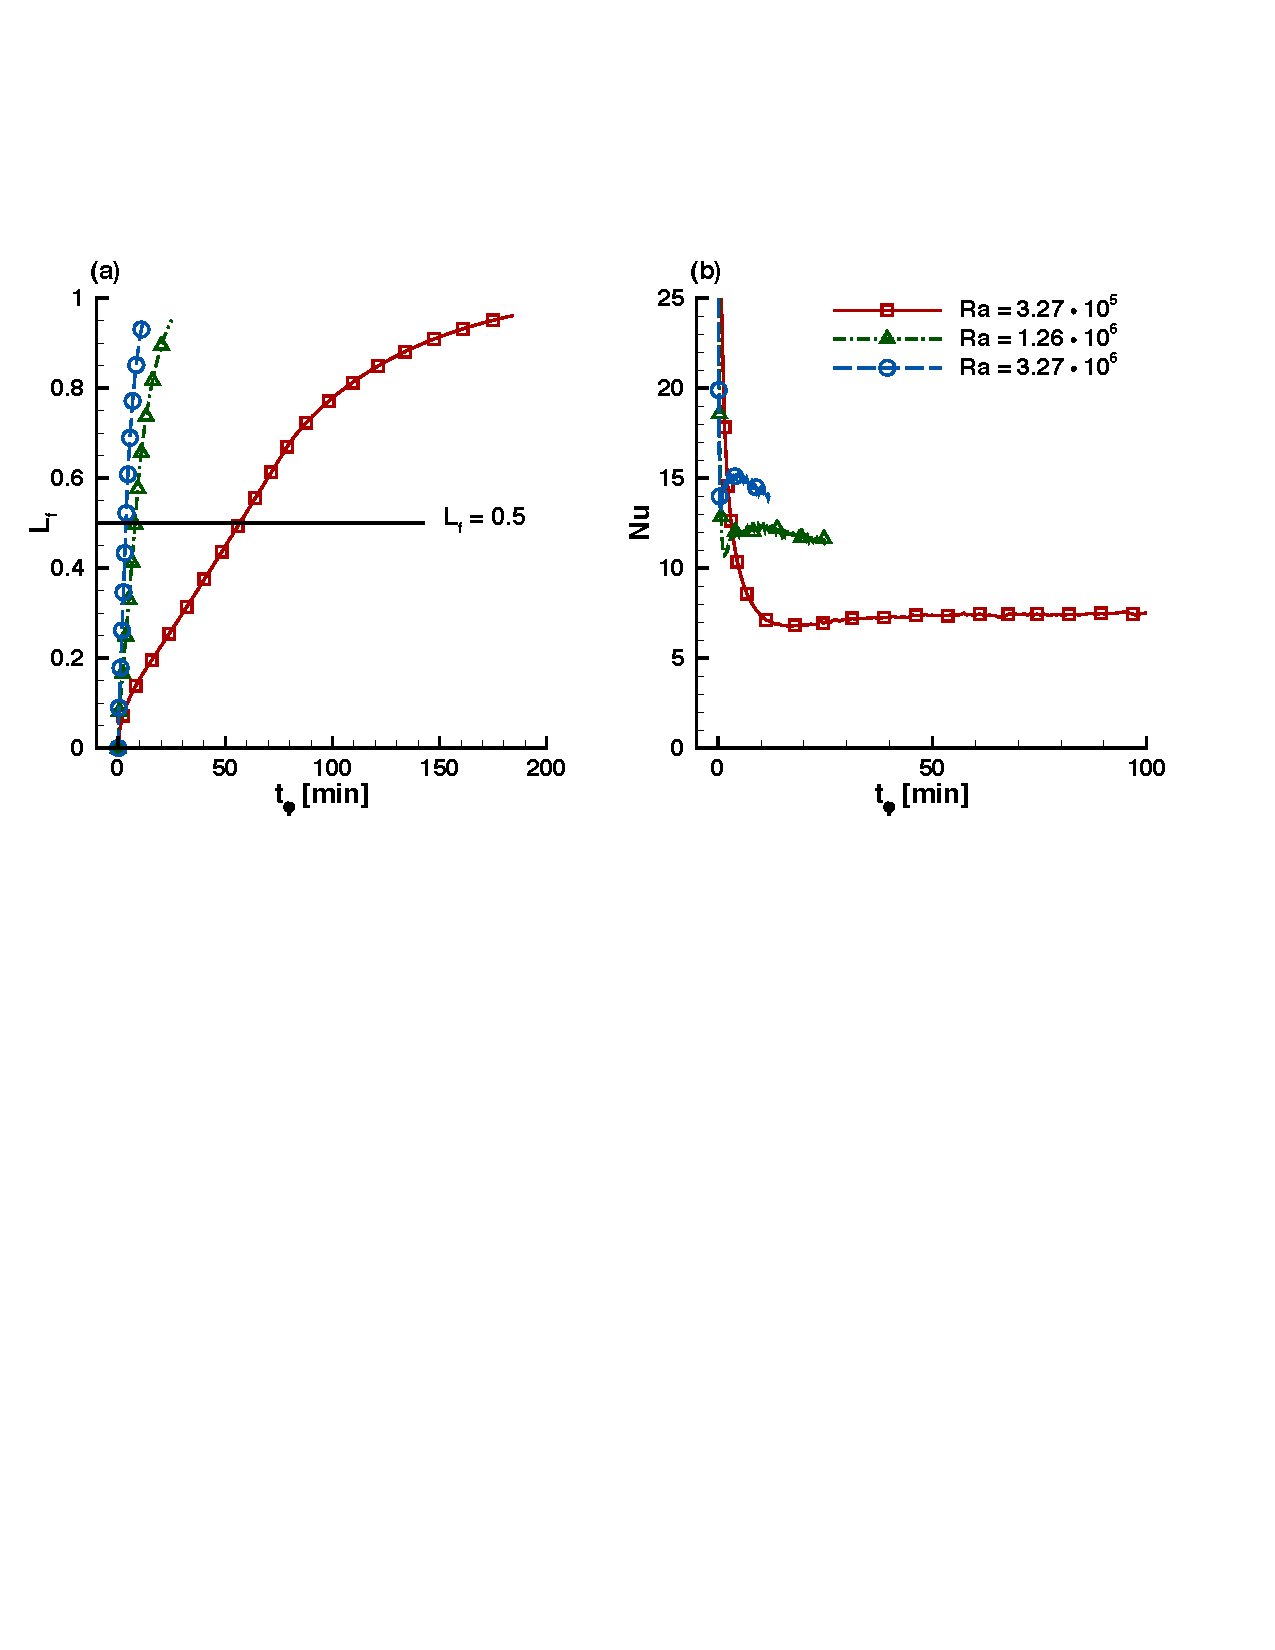
\includegraphics[width=.9\textwidth]{\figpath/Fig_cap_melting/fig09_2}
	\end{center}
	\caption{Complete melting of the PCM.  Influence of the value of the Rayleigh number ($\Ray$) on the time evolution of the liquid fraction (a) and the average Nusselt number defined at the hot (left) wall (b). The reference case ($\Ray=3.27\cdot 10^5$) is represented by red continuous lines. The value of the $\Ray$ and $\Ste$ were increased by a factor of $5$ and $10$, respectively.}\label{fig:Ra-Nusselt-deltaT}
\end{figure}

\newpage
\clearpage
\section{Basal Melting of n-octadecane PCM. Case BM} \label{sec-melting-basal}

We now pay further attention to BM case.
We investigate the melting of pure n-octadecane PCM in a square enclosure subject to heating from the bottom side.
When compared to the lateral melting case, the dynamic of the melting is different for such configuration, in which natural convection develops in the form of B�nard cells. %and results in a non-planar solid-liquid interface. 
The physical parameters and the numerical configuration are reported in Fig. \ref{fig:melt-scheme}.
%Four Rayleigh numbers are carried out: $\Ray = 3.27 \cdot 10^5$, $1.62 \cdot 10^6$, $3.27 \cdot 10^6$, and $6.54 \cdot 10^6$ to assess the influence of the size of the domain on the dynamic of the natural convection flow.
%as observed by \cite{madruga2018dynamic}.
%The PCM is initially solid with isothermal temperature.
%The top of the wall is set at $\theta = \theta_c $, the vertical walls are adiabatic and the bottom wall is heated at a dimensionless temperature $\theta = \theta_h$.
We perform two-dimensional numerical simulations even if 
 \cite{gau1983flow} and  \cite{gong1998flow} have noticed the existence of three-dimensional convection cells during the very first step of the melting process.
These three-dimensional convection cells are however usually neglected for relatively moderate $\Ray$ numbers, mainly for $\Ray \leq 10^8$. 
In such case actually, three-dimensional cells exist in a very short duration compared with the whole melting step,
so that the two-dimensional model is realistic.

\noindent A qualitative description of the dynamic of the natural convection flow and its impact on the melting front is first addressed.
Then, a scale analysis is conducted to describe the heat transfer that occurs during the melting.
Finally, a comparison between LM and BM cases is presented.

%A description of the melting process is presented first, then thorough analysis of the heat transfer through a scale analysis is performed.


\subsection{Time evolution of the melting process} \label{sec-RB-melt-process}
%
%The natural convection flow in the melt PCM during lateral heating exhibits one convection cell deforming the solid-liquid interface (see Fig. \ref{fig:melt-field}).
%The dynamic of the natural convection flow during the basal heating is different,
%since it is known that any non-planar topography can lead to a baroclinic flow at any Rayleigh number.

Fig. \ref{fig:melt-below} displays the structure of the natural convection in the melting PCM through a sequence of panels for temperature isolines and streamlines in the liquid phase, for Rayleigh numbers ranging from $\Ray = 3.27 \cdot 10^5$ to $\Ray = 3.27 \cdot 10^6$, after the primary instability.
An array of lengthening plumes (panel a to c) and counter-rotating convective cells (panel d to f)  are located in the liquid phase,
in which the number of thermal plumes increases with the Rayleigh number.
For $\Ray = 3.27 \cdot 10^5$, one can observe three equidistant plumes and five convective cells in Figs. \ref{fig:melt-below}a and \ref{fig:melt-below}d, while four and six plumes are observed for $\Ray = 1.635 \cdot 10^6$ and $\Ray = 3.27 \cdot 10^6$ respectively (Figs. \ref{fig:melt-below}b and \ref{fig:melt-below}c).
These observations agree well with the numerical results of \cite{gong1998flow} and \cite{madruga2018dynamic} who studied the correlation between the number of thermal plumes and the size of the domain.
The shape of the interface is directly linked to the dynamic of these plumes.
The mushroom form of the plumes results from the two symmetric counter-rotating convective cells surrounding each of them.
We observe an anti-clockwise recirculation of the left convection cell and a clockwise recirculation of the right.
Thus, the melt is heated to the highest temperature at bottom and then floats up, reaches the phase change interface and splits into opposite directions.
The melt is cooled as it flows through the phase-change interface.
It results a non-planar front with a peak at the center of each couple of counter-rotating convective cells.
\begin{figure}
	\begin{center}
		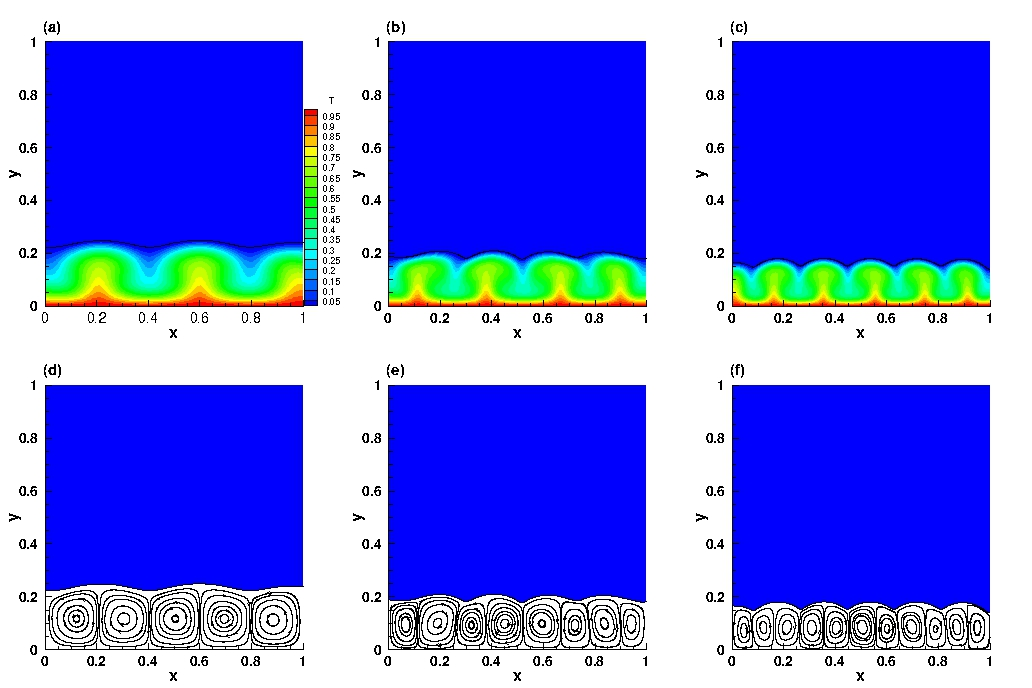
\includegraphics[width=\textwidth]{\figpath/Fig_cap_melting_basal/T_MELT_BASAL_heating_2}
	\end{center}
	\caption{Melting of PCM heated from below. (top) Temperature field and solid-liquid interface for different Rayleigh numbers (a) $\Ray = 3.27 \cdot 10^5$ and $t=30$, (b)  $\Ray = 1.635 \cdot 10^6$ and $t=15$, (c) $\Ray = 3.27 \cdot 10^6$ and $t=10$ (bottom) streamlines in the liquid phase.}
	\label{fig:melt-below}
\end{figure}

\noindent As the melting evolves, it is useful to introduce the effective Rayleigh and Nusselt numbers of the fluid layer, based on the height of the melting PCM, to describe the temporal evolution of the melting:
\begin{eqnarray}
	\Ray_{e} &=& \Ray \times {\bar \delta_H} ^3, \\
	\Nuss_{e} &=& \Nuss \times \bar \delta_H ,
\end{eqnarray}

\noindent with ${\bar \delta_H}$ the non-dimensional averaged fluid height. Note that $\bar \delta_H $ could be assimilated to the liquid fraction.

%\noindent In the limit of vanishing $\Ste$ number, the classical no-slip Rayleigh-B�nard convection predicts a critical Rayleigh number $\Ray_c \approx 1707.76 $ \citep{chandrasekhar2013hydrodynamic} after which the first instability appears. %and the melting front becomes non-planar.
%This critical value is however higher for increasing $\Ste$ numbers.
%In our simulations, the convective onset occurs at around $\Ray_e \approx 5 \times 10^3$, .

\begin{figure}
	\begin{center}
		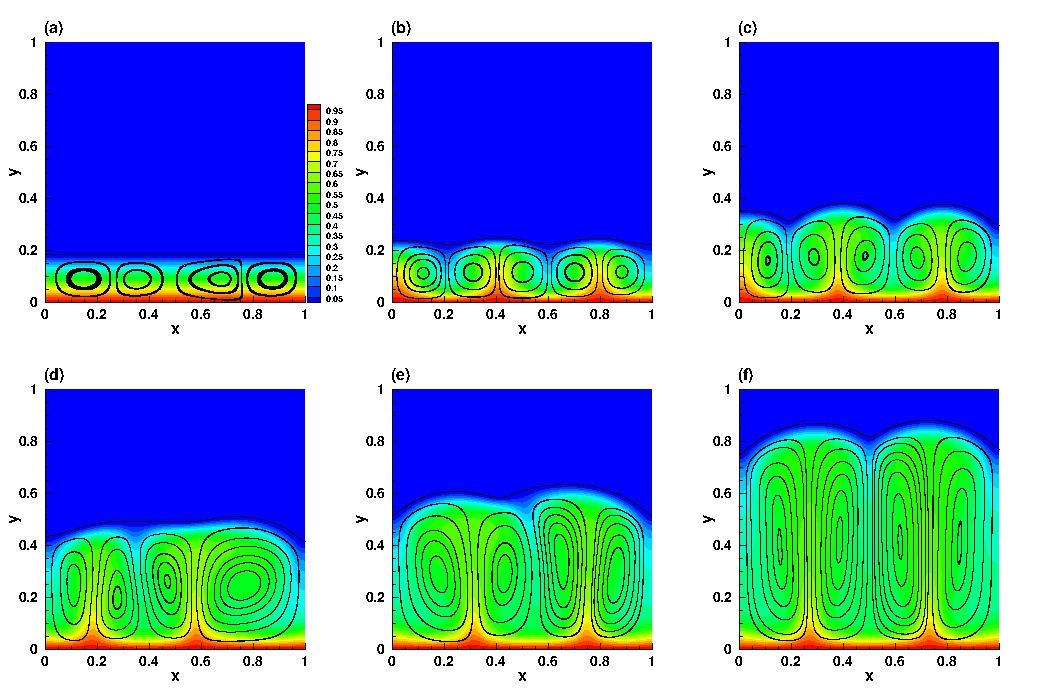
\includegraphics[width=\textwidth]{\figpath/Fig_cap_melting_basal/T_evol_Ra-327e5}
	\end{center}
	\caption{Melting of PCM heated from below for $\Ray = 3.27 \cdot 10^5$. Time evolution of the temperature field, the streamlines and melting fronts corresponding to $6$ effective $\Ray$ numbers:
	$\Ray_e = 2260.65$ (a), $\Ray_e = 4828.42$ (b), $\Ray_e = 1.362 \cdot 10^4$ (c), $\Ray_e = 3.468 \cdot 10^4$ (d), $\Ray_e = 6.925 \cdot 10^4$ (d), and $\Ray_e = 1.97 \cdot 10^5$ (f).}
	\label{fig:T-evol-Ra-3.27e5}
\end{figure}

%The time evolution of the melting for $\Ray = 3.27 \times 10^5$ is illustrated in details through panels (a) to (f) of Fig. \ref{fig:T-evol-Ra-3.27e5}.
Fig. \ref{fig:T-evol-Ra-3.27e5} details the time evolution of the melting for $\Ray = 3.27 \times 10^5$.
Before the first instability arises, the melt layer evolves solely by conduction. 
There is no noticeable fluid flow and the melting front remains straight (panel a).
The convective onset occurs at $\Ray_e \approx 5 \times 10^3$ when the phase-change interface becomes non-planar (panel b), which is in good agreement with the observation of \cite{esfahani2018basal,favier2019rayleigh}.
We note that, in the framework of the classical Rayleigh-B�nard convection flow, in the limit of vanishing $\Ste$ number, the first instability appears at critical Rayleigh number $\Ray_c \approx 1707.76 $.
This critical value is however higher for increasing $\Ste$ numbers.
The appearance of convection is marked by a change in the shape of the interface from straight to nearly periodic curve.

\noindent When the fluid depth increases, the effective Rayleigh number increases and the convective rolls are stretched vertically (panels b and c).
We note that during this stage, the number of rolls is time-independent.
This stage could be compared to the steady convection after the onset in the Rayleigh-B�nard system (see \cite{chandrasekhar2013hydrodynamic}).

\noindent After the rolls are elongated vertically, they start to oscillate laterally and then merge to create greater rolls (panels d and e).
The essential consequence of this observation is that the melting front is modified.
The interface is actually shaped by the new flow pattern. 
%Two peaks are observed but are still periodic at the interface related to the four convective rolls.
Finally, after the roll merging and the oscillating behavior observed in panels (d) and (e), 
the foregoing steady convection observation is then reached again in panel (f).

%\begin{figure}
%	\begin{center}
%		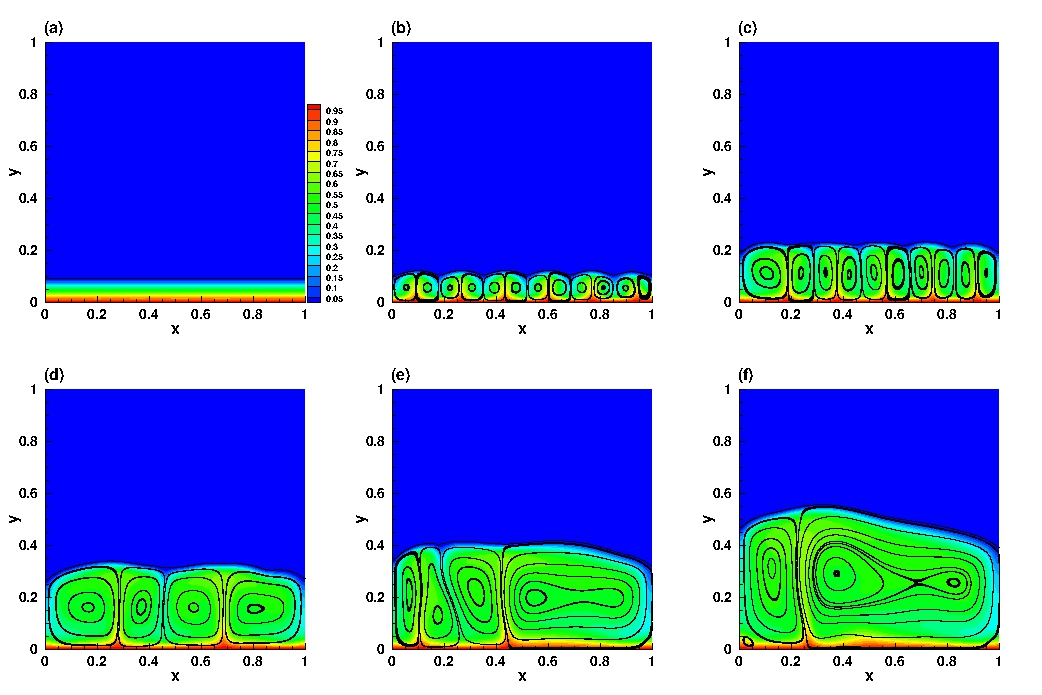
\includegraphics[width=\textwidth]{\figpath/Fig_cap_melting_basal/T_evol_327e6_1}
%		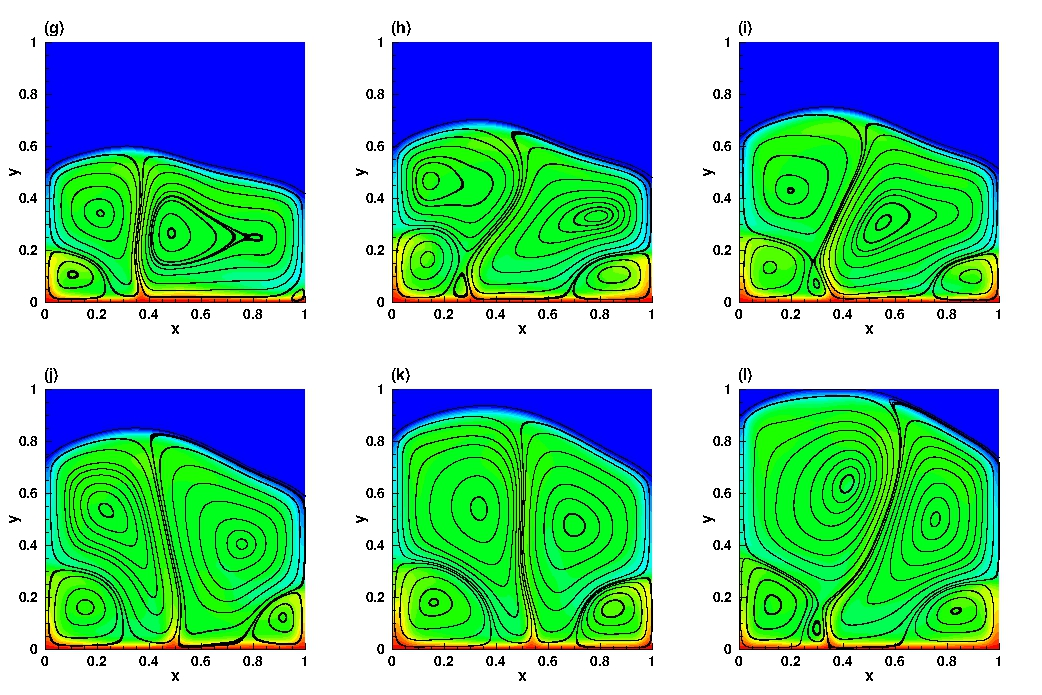
\includegraphics[width=\textwidth]{\figpath/Fig_cap_melting_basal/T_evol_327e6_2}
%	\end{center}
%	\caption{Melting of PCM heated from below: Temperature field and solid-liquid interface for different size of the domain. $\Ray = 3.27 \cdot 10^6$}
%	\label{fig:T-evol-Ra-3.27e6}
%\end{figure}


\begin{figure}
	\begin{center}
		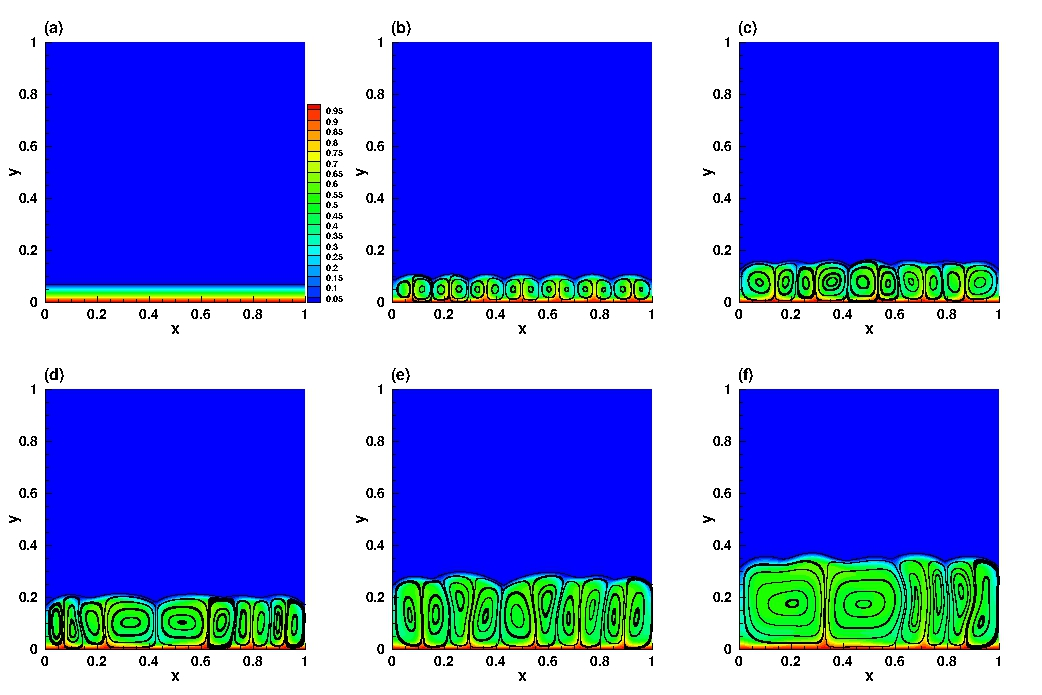
\includegraphics[width=\textwidth]{\figpath/Fig_cap_melting_basal/T_evol_654e6_1}
		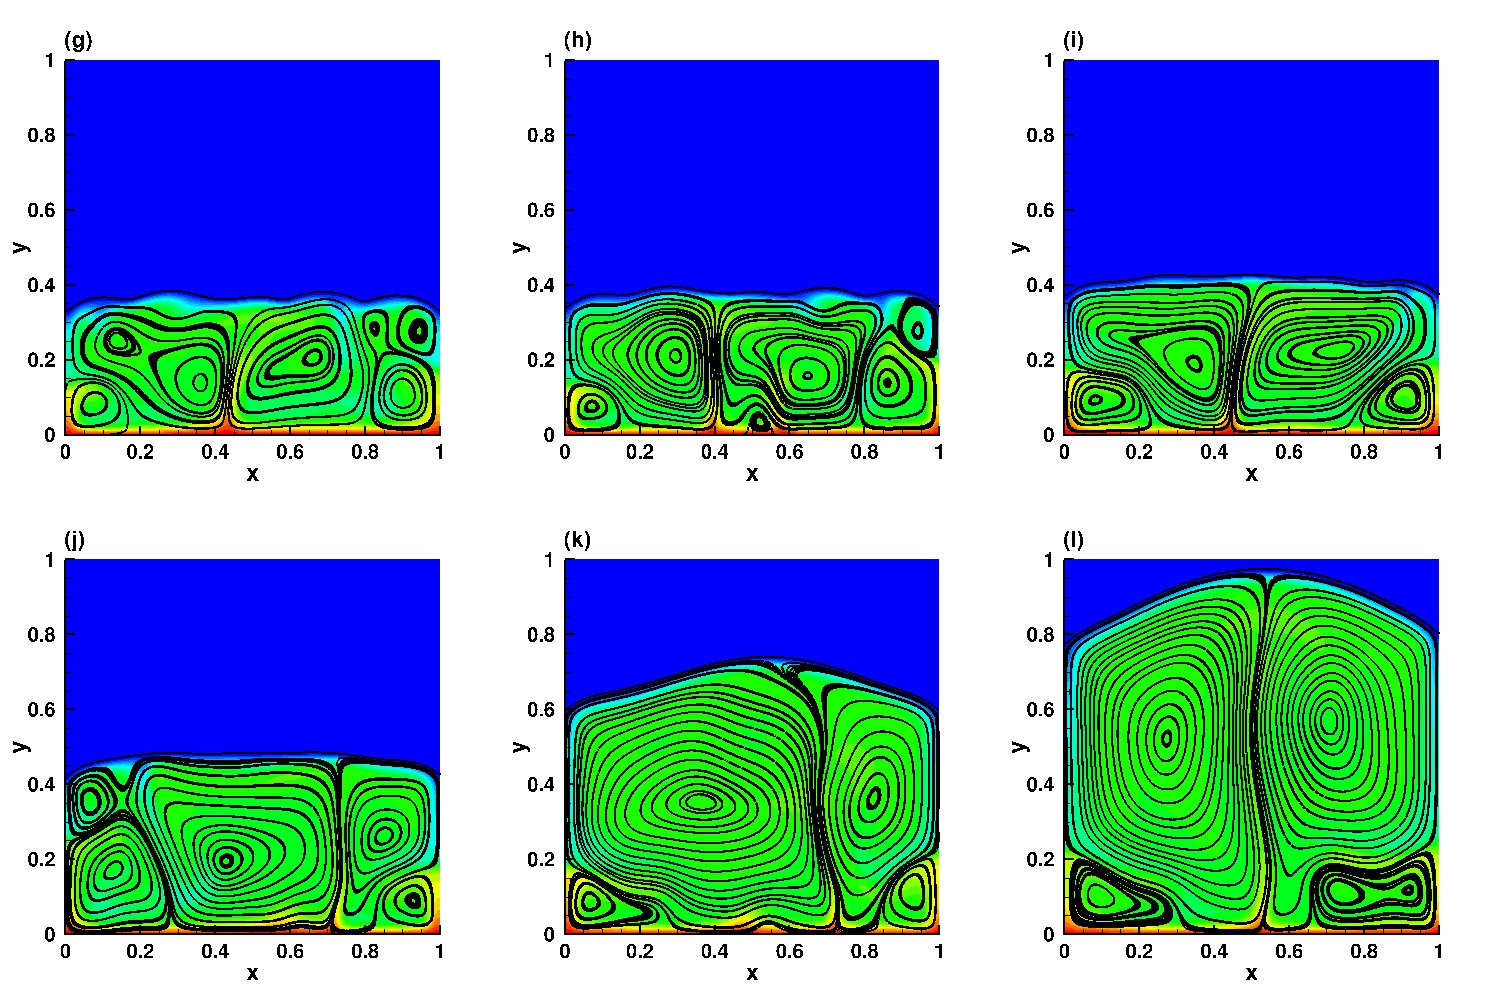
\includegraphics[width=\textwidth]{\figpath/Fig_cap_melting_basal/T_evol_654e6_3}
	\end{center}
	\caption{Melting of PCM heated from below: Temperature field and solid-liquid interface for different size of the domain. $\Ray = 6.54 \cdot 10^6$}
	\label{fig:T-evol-Ra-6.54e6}
\end{figure}

Fig. \ref{fig:T-evol-Ra-6.54e6} shows the dynamic of the melting for higher $\Ray$ number.
The size of the cavity is increased of an order of $3$, corresponding to $\Ray = 6.54 \cdot 10^6$ while the $\Ste$ number remains the same.
The regimes described previously are recovered in panels (a) to (e), mainly the onset of the natural convection at $\Ray_e = 4.8 \cdot 10^3$ followed by an oscillating regime accompanied by a roll merging process.
At $\Ray_e = 4 \times 10^5$ (panel g) the interface loses periodicity and the structure of the rolls becomes disordered.
At this stage, neither the mushroom form of the plumes nor the periodic distribution of the convection cells are no longer observed.

\subsection{Scale analysis} \label{sec-RB-scal-analysis}
We focus in this section on the heat transfer rate during the melting through a scale analysis.
%We conduct in this section a more quantitative analysis by evaluating .
%The same analysis used for the LM case is used to study the heat transfer when BM case is of interest.
The dynamic of the melting for BM case is usually classified into five regimes in the literature: a conductive regime, a linear regime, an oscillating regime, a turbulent regime, and finally an ultimate regime.
The simulations performed in the present work cover the first three regimes.
During the conductive regime, the heat transfer is fully dominated by the conduction. 
The time evolution of the liquid fraction and the Nusselt number could be approximated by the same scaling obtained in Eq. \ref{eq-Nu-Lf-Corr-Lat}.
However, after the onset of the convection, the quasi-steady evolution of the heat transfer for LM case is no longer observed due to non-linear instabilities.

When the convective heat transfer is fully developed in the melted PCM, two heat transfer process could be identified.
Firstly, a bulk heat transfer process occurs for low effective Rayleigh number regime, mainly for $\Ray_{e} \leq 10^5$.
Secondly, a boundary layer heat transfer regime is predominant when oscillating or turbulent regimes are achieved.
We develop in this section a scale analysis during the linear regime, during which bulk heat transfer occurs, to approximate the amount of heat transfer.
Beyond this regime, due to the important non-linearities of the dynamics, we rely on theories developed in the frame of turbulent Rayleigh-Benard convection flow  \citep{malkus1954heat,grossmann2000scaling}. %made in the frame of Rayleigh-B�nard convection flow
\begin{figure}
\centering
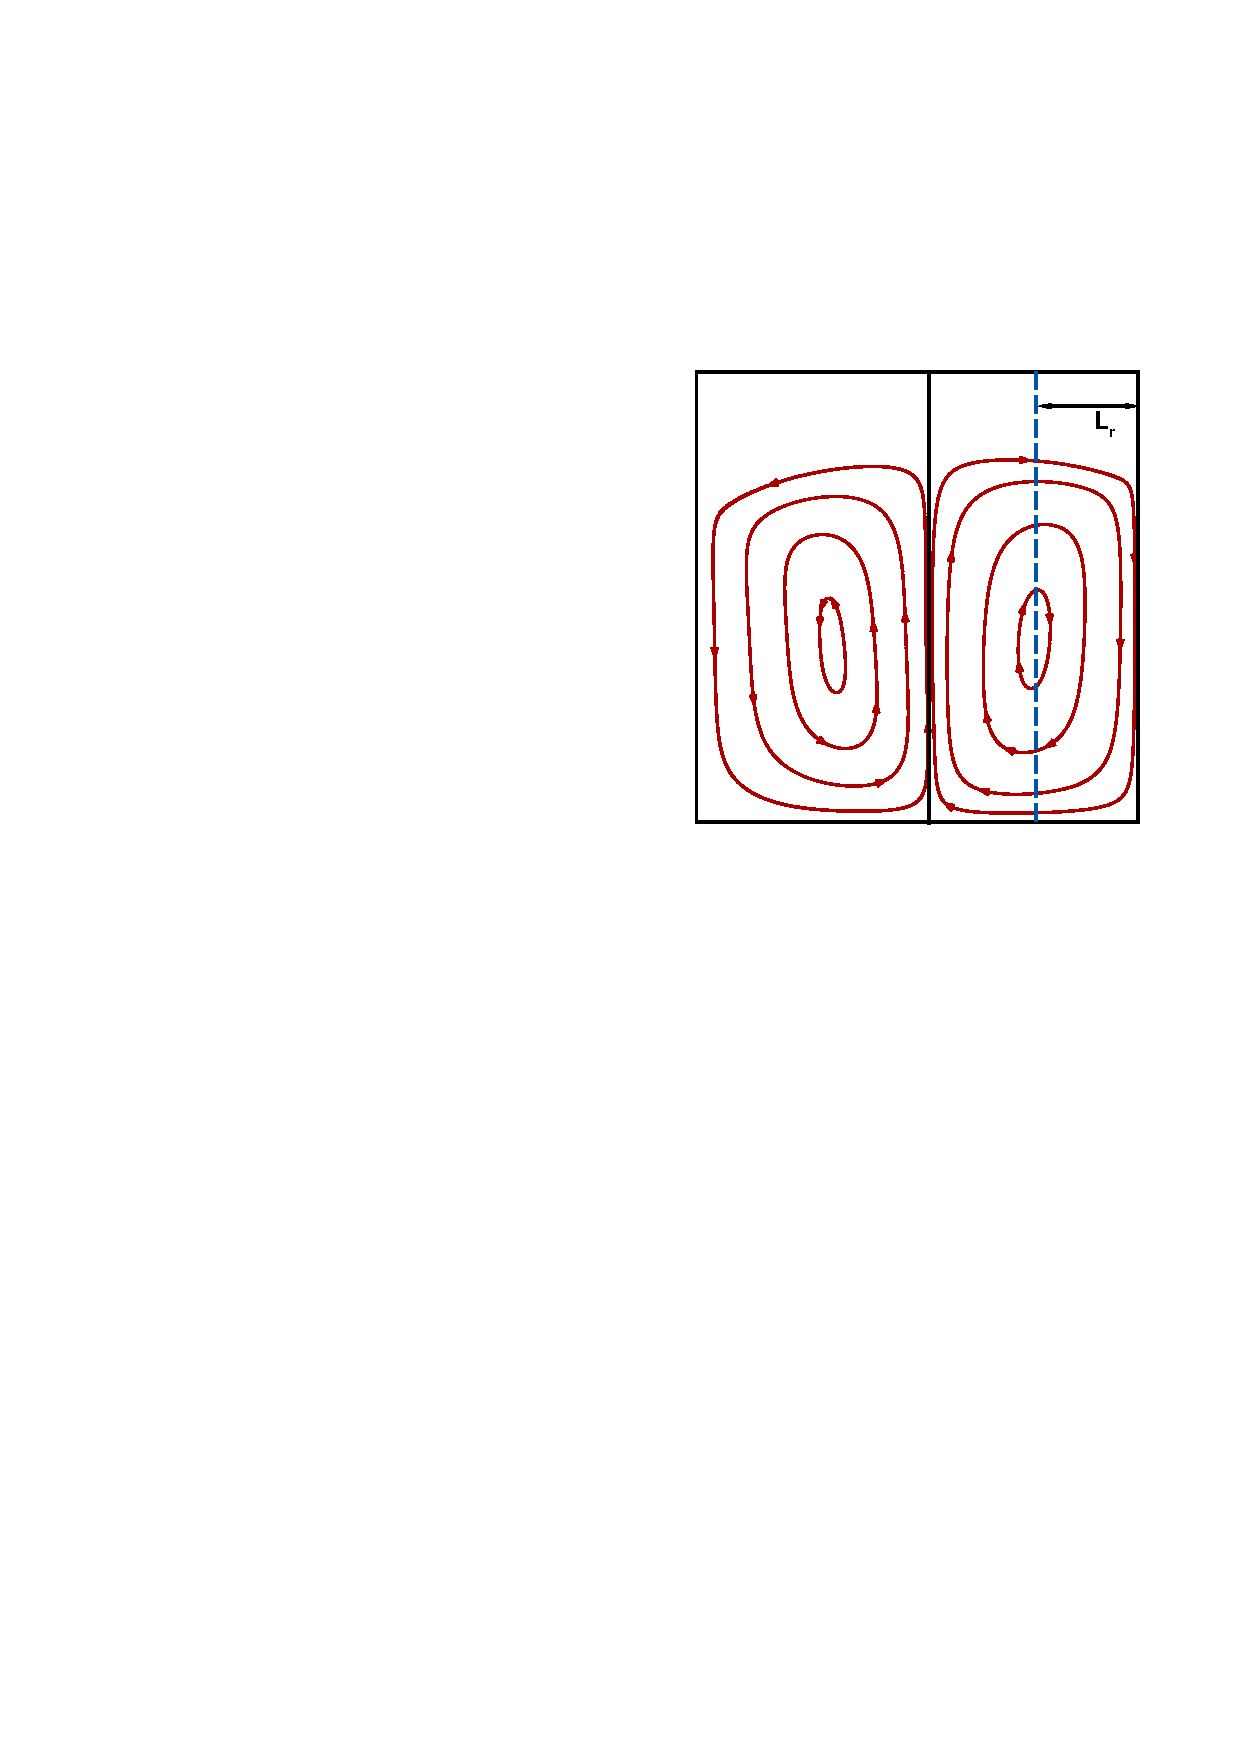
\includegraphics[width=0.5\textwidth]{\figpath/Fig_cap_melting_basal/MELT_basal_rolls}
\caption{Natural convection flow for melting heated from below.}
\label{fig:roll-basal-heating}
\end{figure}

During the linear regime, the convective cells are elongated vertically and the number of rolls is time-independent.
A schematic overview of the phenomenon is drawn in Fig. \ref{fig:roll-basal-heating}. 
Let $L_r$ define the (dimensionless) half-thickness of a cell. 
A good scaling during this regime is hence
\begin{equation}
	x \sim L_{r}, \quad y \sim \bar \delta_H,
\end{equation}

\noindent with $L_{r} \ll \bar \delta_H$.
We consider the dimensionless system of Eqs. \ref{eq-qmvt}  \ref{eq-energ} in the fluid ($C=K=1$, and $S(\theta) = A(\theta) = 0$), which could be rewritten as follows using scaling Eq. \ref{eq-def-scal-1} (i.e. $\Rey = 1$):

\begin{eqnarray} \label{eq-mass-basal}
	\frac{\partial u}{\partial x} + \frac{\partial v}{\partial y} &=& 0, \\  \label{eq-mom-basal-x}
	\frac{\partial u}{\partial t} + u \frac{\partial u}{\partial x} + v \frac{\partial u}{\partial y} &=& - \frac{\partial p}{\partial x} +  \left( \frac{\partial^2 u}{\partial x^2} + \frac{\partial^2 u}{\partial y^2} \right), \\ \label{eq-mom-basal-y}
	\frac{\partial v}{\partial t} + u \frac{\partial v}{\partial x} + v \frac{\partial v}{\partial y} &=& - \frac{\partial p}{\partial y} +   \left( \frac{\partial^2 v}{\partial x^2} + \frac{\partial^2 v}{\partial y^2} \right) + \frac{\Ray}{\Prd} \theta, \\ \label{eq-bound-energy}
	\frac{\partial \theta}{\partial t} + u \frac{\partial \theta}{\partial x} + v \frac{\partial \theta}{\partial y} &=& \frac{1}{\Prd} \left( \frac{\partial^2 \theta}{\partial x^2} + \frac{\partial^2 \theta}{\partial y^2} \right). 	
\end{eqnarray}

\noindent The pressure $p$ is first eliminate by combining $\partial/\partial y$ of Eq. \ref{eq-mom-basal-x} and $\partial/\partial x$ of Eq. \ref{eq-mom-basal-y}, and we have

\begin{eqnarray} \label{eq-mom-rassembly}
	\frac{\partial}{\partial y} \left( \frac{\partial u}{\partial t} + u \frac{\partial u}{\partial x} + v \frac{\partial u}{\partial y} \right) - \frac{\partial}{\partial x} \left(  \frac{\partial v}{\partial t} + u \frac{\partial v}{\partial x} + v \frac{\partial v}{\partial y} \right)  \\ \nonumber
	=  \left[ \frac{\partial}{\partial y} \left( \frac{\partial^2 u}{\partial x^2} + \frac{\partial^2 u}{\partial y^2} \right)   - \frac{\partial}{\partial x} \left( \frac{\partial^2 v}{\partial x^2} + \frac{\partial^2 v}{\partial y^2} \right) \right] - \frac{\Ray}{\Prd} \frac{\partial \theta}{\partial x}.
\end{eqnarray}

\noindent Since we have $L_{r} \ll \bar \delta_H$ (consequently $\partial^2 v/\partial y^2 \ll \partial^2 v/\partial x^2 $),
three terms dominate the Eq. \ref{eq-mom-rassembly}:
\begin{equation}
	\underbrace{\frac{\partial ^2 v}{\partial x \partial t}}_{inertia} \quad \underbrace{ \frac{\partial^3v}{\partial x^3}}_{friction} \quad \underbrace{\frac{\Ray}{\Prd} \frac{\partial \theta}{\partial x}}_{buoyancy}.
\end{equation}

\noindent In terms of representative scales, this momentum balance reads
\begin{equation} \label{eq-basal-heat-mom}
	\underbrace{\frac{v}{L_{r} t}}_{inertia} \quad \underbrace{\frac{v}{L_{r}^3}}_{friction} \quad \underbrace{\frac{\Ray}{\Prd} \frac{\delta \theta}{L_{r}}}_{buoyancy},
\end{equation}

\noindent with $\delta \theta = 1$. The regime of interest occurs after a pure conductive regime where the boundary layer thickness increases as
\begin{equation}
	\delta_{\theta} \sim \left( \frac{t}{\Prd} \right)^{1/2}.
\end{equation}

\noindent Since the heat transfer is dominated solely by bulk heat transfer we have
\begin{equation} \label{eq-Lf-deltT}
 	L_{r} \sim \delta_{\theta}.
 \end{equation}
 
\noindent Eq. \ref{eq-basal-heat-mom} could be hence simplified by replacing $\delta_{\theta}^2 \sim \left(\frac{t}{\Prd}\right)$ and dividing Eq. \ref{eq-basal-heat-mom} through the friction scale, leading to
\begin{equation}
	\underbrace{\frac{1}{\Prd}}_{inertia} \quad \underbrace{1}_{friction}  \quad \underbrace{\frac{\Ray \delta_{\theta}^2}{v \Prd}}_{buoyancy}.
\end{equation}

\noindent For high-Prandtl fluid, the momentum balance is between buoyancy and friction and we obtain
\begin{equation}
	v \sim \frac{\Ray \delta_{\theta}^2}{\Prd}.
\end{equation}

Next, we turn attention back to the energy Eq. \ref{eq-bound-energy} and identify
three distinct effects:
\begin{equation}
	\underbrace{\frac{1}{t}}_{Inertia} \quad \underbrace{\frac{v}{\bar \delta_H}}_{Convection} \quad \underbrace{\frac{1}{L_r^2 \Prd}}_{Conduction}.
\end{equation}

\noindent When $t$ increases, there comes an effective time $t_{e}$ where the inertia decreases in importance and the energy equation expresses a balance between the convection and the conduction heat transfer,
%Again, if the assumption $L_r \sim \delta_T$ holds, we obtain:
\begin{equation}
	\frac{v}{\bar \delta_H} \sim \frac{1}{\delta_{\theta}^2 \Prd},
\end{equation}

\noindent leading to
\begin{equation}
	t_{e} \sim \left( \frac{\bar \delta_H}{\Ray_e} \right)^{1/2} \times \Prd.
\end{equation}

\noindent At such a time, the thermal layer thickness is:
\begin{equation}
	\delta_{\theta} \sim \left(\frac{t_{e}}{\Prd} \right)^{1/2} \sim \left(\frac{\bar \delta_H}{ \Ray_{e}}\right)^{1/4} \sim \left( \bar \delta_H \right)^{-1/2} \Ray^{-1/4}.
\end{equation}

\noindent Accordingly, for $\Ray \leq 10^5$, the scaling for $\Nuss$ could be written as

\begin{equation} \label{eq-Nu-scal-basal}
	\Nuss \sim  \delta_H ^{1/2} \times \Ray^{1/4}.
\end{equation}

%\noindent One can note that when $\bar \delta_H = H$, we recover the scaling for LM case in Eq. \ref{eq-Nu-Ra-LM}.

\noindent Fig. \ref{fig:NU-LF-evol}a plots the temporal evolution of the heat flux, represented by the Nusselt number, and the strength of buoyancy, represented by the Rayleigh number, when the melting evolves.

\noindent The onset of the convection arises at $\Ray_e = 3 \times 10^3$, when a sudden jump in $\Nuss_e$ is observed.
\cite{vasil2011dynamic} have investigated a weakly non-linear stability analysis and have highlighted a superexponentional amplitude growth when the Rayleigh number becomes close to the traditional critical value in the limit of vanishing Stefan number.
This superexponential growth is moreover followed by a rapid pattern readjustment.
The trend of $\Nuss_e$ at the onset of convection is in total accordance with this prediction of \cite{vasil2011dynamic}.
The results of \citep{esfahani2018basal,madruga2018dynamic,favier2019rayleigh} exhibit the same trend despite the different boundary conditions (periodic lateral boundary conditions, adiabatic boundary conditions at the top of the cavity, and low value of $\Prd$ for \cite{esfahani2018basal} and \cite{favier2019rayleigh}).

\noindent The rapid growth of $\Nuss_e$ is followed by a power law with averaged exponent $\Nuss \sim \Ray^{0.28}$ for  $10^3 \leq \Ray \leq  10^5$.
Our results overestimate slightly the predicted scaling exponent of $1/4$ presented in Eq. \ref{eq-Nu-scal-basal}.
This is mostly due to the number of convection cells in the melted PCM, which increases with the $\Ray$ numbers, and the effect of the non-planar solid-liquid interface, not taken into account in our analysis.
However, our numerical results match better with the Grossmann-Lohse theory \citep{grossmann2000scaling}, which predicts a scaling exponent of $2/7$, within the framework of natural convection flow.

\noindent Finally, the transition from steady pattern of the convective rolls to oscillating pattern followed by cell merging, as it is clearly shown in Fig. \ref{fig:T-evol-Ra-6.54e6}(d-f), 
is also illustrated by a decrease of $\Nuss$ at $\Ray \sim 10^5$ followed by high oscillation in the temporal evolution of the heat transfer.
The power-law relation $\Nuss-\Ray$ is bounded in this stage by the average exponent of $1/3$.

\begin{table}[!ht]
   \begin{center}
      \begin{tabular}{*{3}{cl}}
         $\Ray$ & Linear regime & oscillating regime \\
         \bottomrule
         $3.27 \cdot 10^5$ & $0.286299$ & - \\
         $1.635 \cdot 10^6$ & $0.274789$ & 0.269158 \\
         $3.27 \cdot 10^6$ & $0.279616$ & 0.283658 \\
         $6.54 \cdot 10^6$ & $0.274043$ & 0.294528 \\
      \end{tabular}
   \end{center}
   \caption{Exponent of the power laws of the linear and the oscillating regimes.}
   \label{tab-power-expo}
\end{table}

As far as the time evolution of the liquid fraction $L_f$ is concerned, one can introduce the following scaling, from the \cite{grossmann2000scaling} theory (see also \cite{favier2019rayleigh}):
\begin{equation}\label{eq:scal-Lf-RB}
	L_f(t) = \left[ \sqrt{2 t}^{(2-3 \beta)}+ c \Ray^\beta t \right]^{1/(2-3 \beta)},
\end{equation}
with $\beta$ the exponent in the $\Nuss-\Ray$ power law, $c = \frac{(2-3 \beta) \gamma}{2 + \Ste}$ and $\gamma$ a constant fitted from numerical data.

The time evolution of the liquid fraction is illustrated in Fig. \ref{fig:NU-LF-evol}b.
As expected, the purely diffusive stage displays the scaling $L_f \sim t^{1/2}$.
Replacing $\beta$ by the exponent value $2/7$ in Eq. \ref{eq:scal-Lf-RB}, we obtain $L_f \sim t^{7/8}$.
Our simulations exhibit a power-law evolution of $L_f \sim t^{0.82}$ when the convection is fully developed in the fluid, corresponding to $\Ray_e \geq \Ray_c$.


\begin{figure}
	\begin{center}
		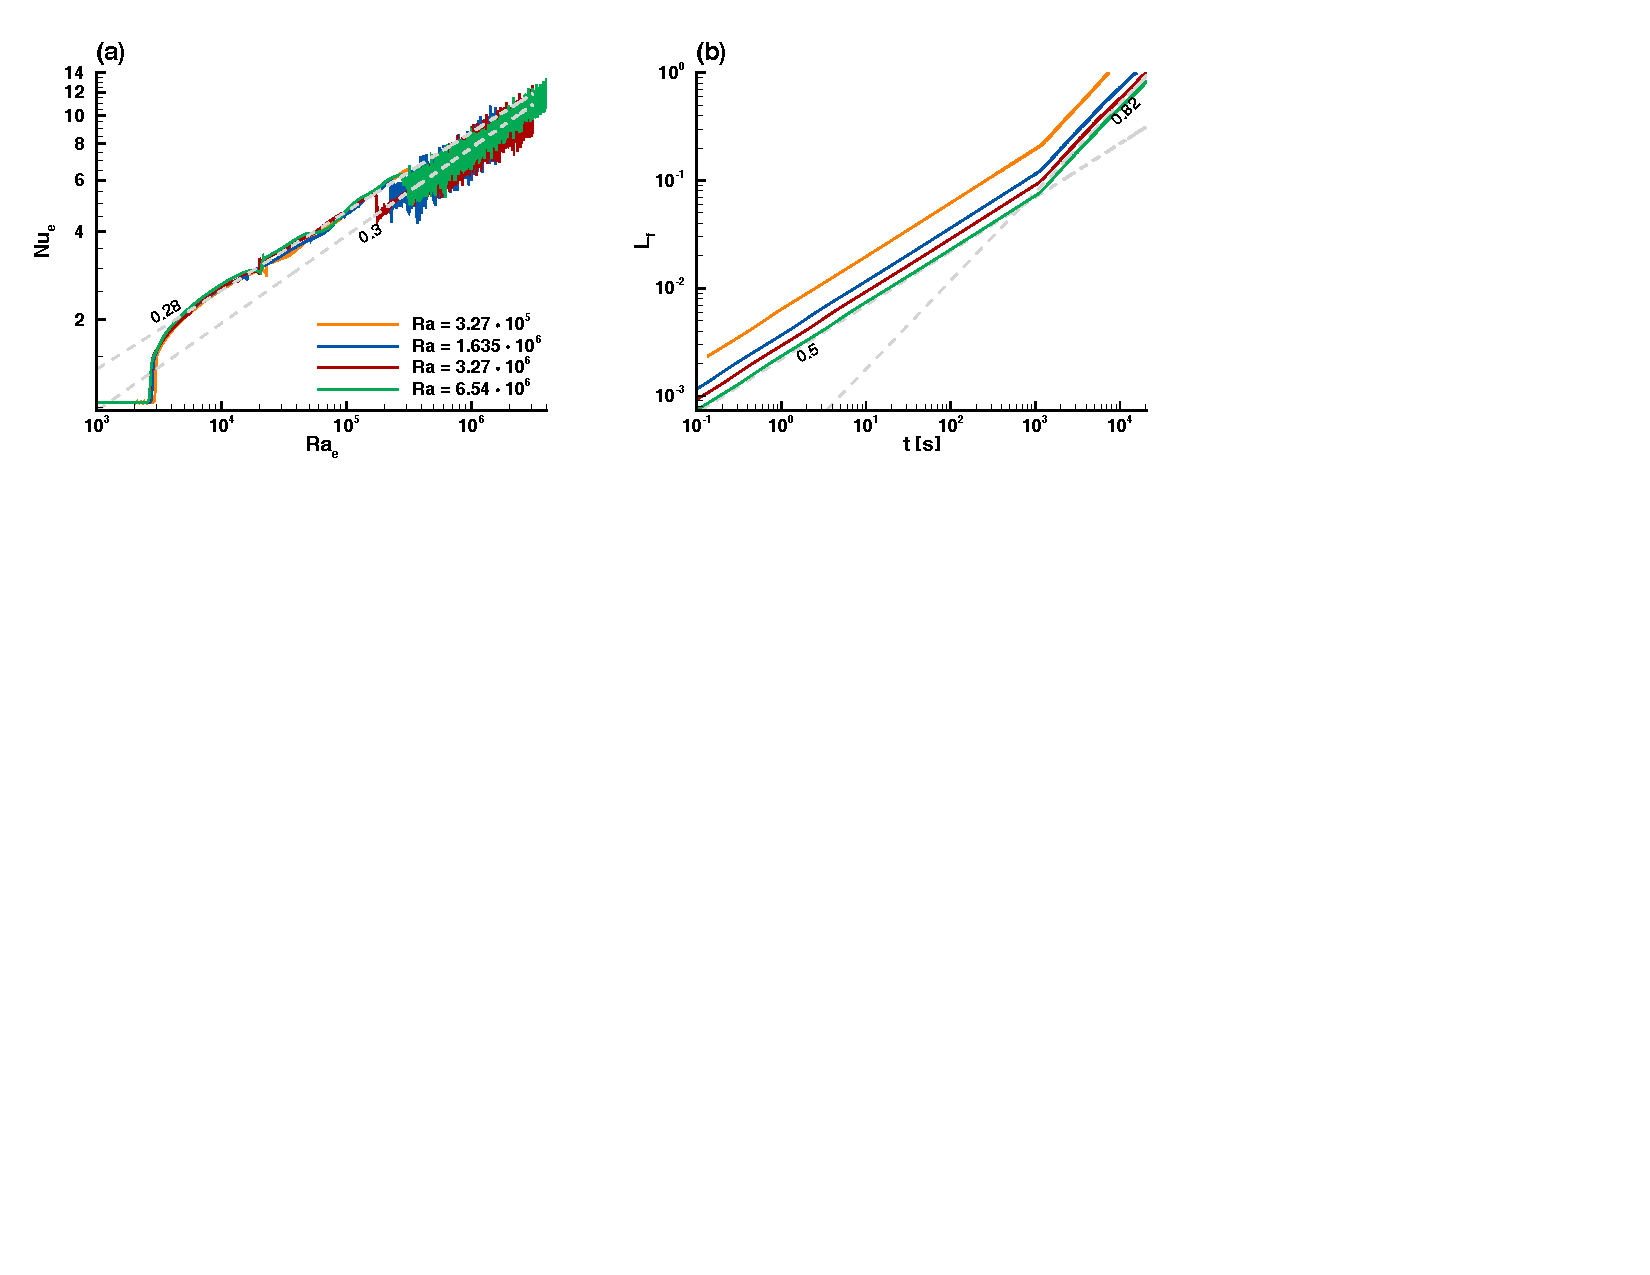
\includegraphics[width=\textwidth]{\figpath/Fig_cap_melting_basal/NU-LF-PHYS_2}
	\end{center}
	\caption{BM case for three Rayleigh numbers: $\Ray = 3.27 \cdot 10^5$, $1.62 \cdot 10^6$, and $3.27 \cdot 10^6$. Time evolution of the Nusselt number (a) and the melting rate (b).}
	\label{fig:NU-LF-evol}
\end{figure}

\section{Comparison between LM and BM cases} \label{sec-compare-LM-BM}
We now compare the temporal evolution of some physical quantities for both cases LM and BM.
The liquid fraction $L_f$, the Nusselt number $\Nuss$, and the accumulated heat input $Q_0$ are plotted in Fig. \ref{fig:NU-LF-Q0-compare}, for $3$ values of the $\Ray$ numbers: $\Ray = 3.27 \cdot 10^5$ (left), $\Ray = 1.62 \cdot 10^6$ (middle), and $\Ray = 3.27 \cdot 10^6$ (right).
Blue lines denote the lateral heating case and red lines the basal heating.

The temporal evolution of melting rate, the heat transfer rate, and the accumulated heat input, for $\Ray = 3.27 \cdot 10^5$ are reported in the left column of Fig. \ref{fig:NU-LF-Q0-compare}.
%For $\Ray = 3.27 \cdot 10^5$ (panel a), $L_f$, $\Nuss$, and $Q_0$ evolves with the same trends.
From $t=0$ to $t=18$, red and blue curves matches perfectly well during the conductive regime. 
It is the expected solution since the scaling analysis performed previously have predicted the same trend for both cases during the conductive regime.
Differences occur from the emergence of the convective flow at $t=20$.
The evolution of $\Nuss$ is smooth for LM case, while the BM case exhibits a sudden increase due to the hydrodynamical instabilities. 
The gap between both curves is then followed by a reconnection at $t=40$.
As predicted by Eq. \ref{eq-Nu-scal-basal}, as the fluid depth $\bar \delta_H$ increases, the behavior of the heat transfer occurring during BM case should tend to the LM case value, during the linear regime.

Significant differences arise for $\Ray_e \geq 5 \cdot 10^5$, corresponding to greater cavity size. 
%From $t=$ $\Ray = 1.62 \cdot 10^6$, and $\Ray = 3.27 \cdot 10^6$.
From $t=40$ for $\Ray = 1.62 \cdot 10^6$ (panel b), and $t=30$ for $\Ray = 3.27 \cdot 10^6$ (panel c), $\Nuss$ displays a highly oscillating value, for the BM case, when the melting advances, while smooth and quasi-steady evolution is noticed for the LM case.
%noticeable differences are apparent in the time evolution of the Nusselt number.
%The blue curves (lateral heating) exhibit a smooth and a quasi-steady evolution of $\Nuss$, while high oscillating value of $\Nuss$ is observed for the red curves (basal heating).
Moreover, lower amount of heat transfer and accumulated heat input is featured by the BM case.
At this stage, the decrease of the heat transfer is correlated by the decrease of the number of convection cells.
%the decrease of the number of convection cells is accompanied by a decrease of the heat transfer.
It occurs when the heat transfer is no longer bulk transfer for the BM case.
%Consequently, the accumulated heat input $Q_0$ is higher for the LM case from the oscillating regime.

\noindent This decreasing value of $Q_0$ and $\Nuss$, for the BM case, during the oscillating regime, could be explained by the rule of the bulk heat transfer at this stage.
The scaling relation in Eq. \ref{eq-Lf-deltT} is indeed no more valid, since $\delta_{\theta} \ll L_r$.
Thus, the contribution of the bulk part during the oscillating regime is:
\begin{equation} \label{eq-Nu-scal-bulk}
	\Nuss \sim \left( \frac{H}{L_r}\right)^{1/4} \Ray^{1/4},
\end{equation}

\noindent which indicates clearly that higher is the size of the convective cells, lower is the amount of the bulk heat transfer.
One can note that, when $L_r = H$ we recover the Nusselt scaling for natural convection in vertically heated square cavity case.

%When the boundary layer heat transfer is predominant, Eq. \ref{eq-Lf-deltT} is indeed no more valid, and the contribution of 

\begin{figure}
	\begin{center}
		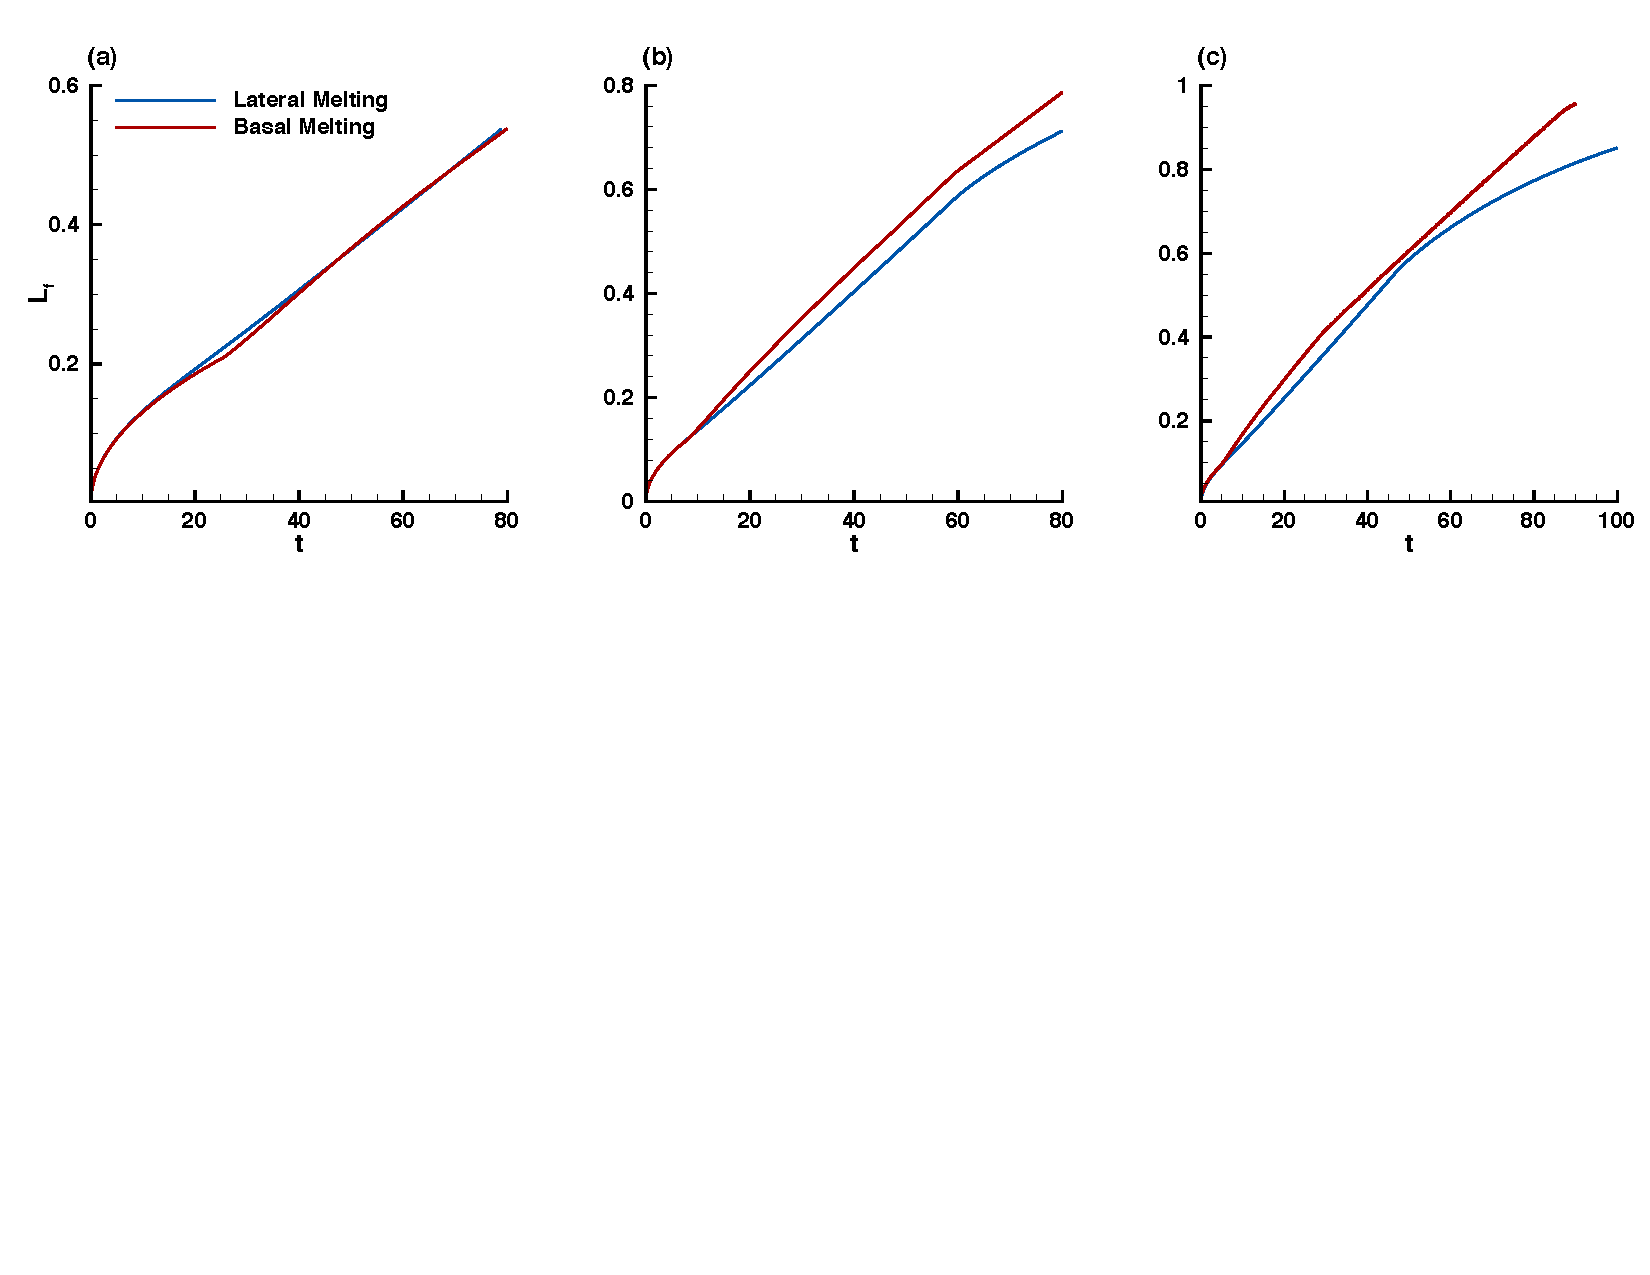
\includegraphics[width=\textwidth]{\figpath/Fig_cap_melting_basal/Lf-COMPARE}\\
		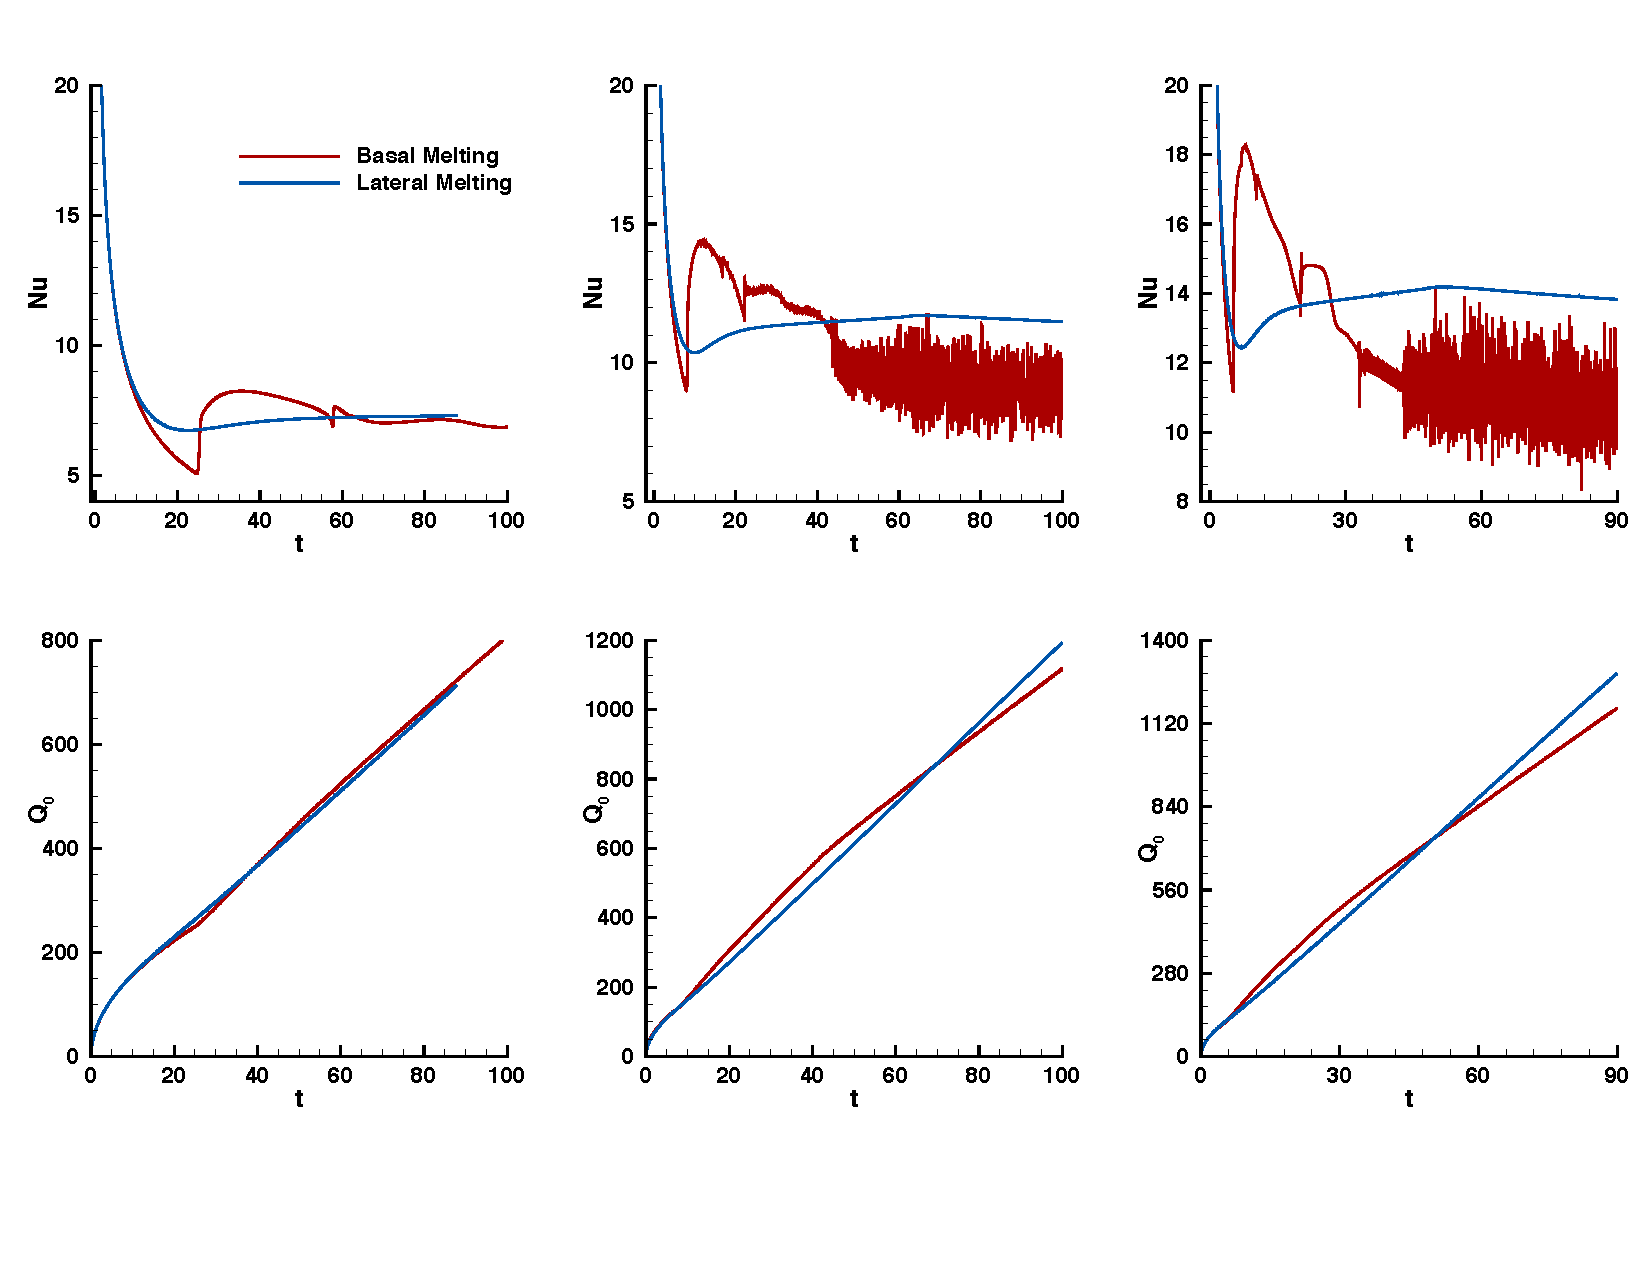
\includegraphics[width=\textwidth]{\figpath/Fig_cap_melting_basal/Nu-Q0-COMPARE}
	\end{center}
	\caption{Comparison of different physical quantities during lateral and basal melting for (a) $\Ray = 3.27 \cdot 10^5$, (b)  $\Ray = 1.62 \cdot 10^6$, and (c) $\Ray = 3.27 \cdot 10^6$. (top) Liquid fraction, (middle) Nusselt number, and (bottom) accumulated heat input.}
	\label{fig:NU-LF-Q0-compare}
\end{figure}


